%
% TU/e Style Master Thesis template for LaTeX
%
% Public version 1.0
% 2010 - 2013 Thijs Nugteren and Joos Buijs
%
% THIS IS THE MAIN FILE (i.e. compile this file, compiling the others directly won't work)
%

\documentclass[a4paper,10pt,twoside]{report}

%all the other includes etc. are done in the thesis.sty file.
\usepackage{thesis}

%
% These commands need to be defined in order to produce a correct and personalized document
%
\newcommand{\shortdoctitle}{Master's Thesis}
\newcommand{\doctitle}{Inter-case Resource Dependencies}
\newcommand{\docsubtitle}{Master Thesis}

\newcommand{\me}{M.A.W. de Roode, BSc}
\newcommand{\keywords}{resource, inter-case, dependency}
\newcommand{\version}{version 1.1}
\newcommand{\monthYear}{July (2018)}

%Be sure to use all the titles for your committee members!!! (their names show up on the very first page!)
\newcommand{\firstCommitteeMember}{prof. dr. ir. D. Fahland}
\newcommand{\secondCommitteeMember}{}
\newcommand{\thirdCommitteeMember}{}

\author{\me}

%
% PDF settings
%
\hypersetup
{
    pdfauthor={\me},
    pdftitle={\shortdoctitle},
    pdfsubject={\doctitle},
    pdfkeywords={\keywords}
}

\begin{document}

%use this include for PDF and distribution versions
\pagenumbering{roman}
\begin{titlepage}
\begin{center}

\includegraphics[height=2cm]{figures/tue-logo-high}\\
%\LARGE
%Eindhoven University of Technology \\
\large
Department of Mathematics and Computer Science  \\
Architecture of Information Systems Research Group

\vspace*{10cm}

\setlength{\TPHorizModule}{1mm}
\setlength{\TPVertModule}{\TPHorizModule}
% Set the Paragraph Indent to zero, so the first line is not Indented
% Back-up the current value so it can be put back at the end of the title page
\newlength{\backupparindent}
\setlength{\backupparindent}{\parindent}
\setlength{\parindent}{0mm}			
% Begins a textbox at 72 mm from the left of the edge of the paper and 89 mm from the top
% The width of the textbox is 95 mm (167 - 72 mm)
% The height of the box cannot be defined, so it is your task to keep the text not too long
\begin{textblock}{95}(62,89)
    \vspace*{1mm}
    \huge
    \textbf{\doctitle \\}
    \Large
    \vspace*{5mm}
    \textit{\docsubtitle}\\
    \vspace*{10mm}
    \Large
    \me\\
\end{textblock}

\large
Supervisors:\\
\begin{tabular}{rl}
    \firstCommitteeMember\\
    \secondCommitteeMember\\
    \thirdCommitteeMember\\
\end{tabular}

\vfill
\version

\vfill
%\docdate \\
\large
Eindhoven, \monthYear\\

% Put the Paragraph Indent back to its original value
\setlength{\parindent}{\backupparindent}
\end{center}
\end{titlepage} 

\normalsize

\clearemptydoublepage

%Sometimes line numbers are nice, uncomment the next line to enable:
%\linenumbers

%It could be handy to have a list of todos and brainstorms in your thesis
%\chapter*{*General todos*}\todo{remove this chapter}
%\input{chapters/general_todos}

%\chapter*{*Brainstorm results*}\todo{remove this chapter}
%\input{chapters/brainstorm_results}

\chapter*{Abstract}\label{chapter:abstract}
\input{chapters/abstract}

\clearemptydoublepage

%An executive summary if you want:
%\chapter*{Executive summary}\label{chapter:executive_summary}
%\input{chapters/executive_summary}

%\clearemptydoublepage


% \chapter*{Preface}\label{chapter:preface}
% Please write all your preface text here. If you do so, don't forget to thank your supervisor, other committee members, your family, colleagues etc.\ etc. 

\clearemptydoublepage

\tableofcontents

\clearemptydoublepage

\listoffigures

\clearemptydoublepage

\listoftables

\clearemptydoublepage

\lstlistoflistings

\clearemptydoublepage

\chapter{Introduction}\label{chapter:introduction}
\setcounter{page}{0}
\pagenumbering{arabic}
%from here on, start the 'real' page numbering, from 1, with normal digits
\todo{add introduction of subject and research area}



% As is discussed in section \ref{sec:processmining}, there exist many approaches for analysing process performance, but there are no approaches which specifically focus on resources. \todo{Move process mining chapter}

\section{Business Process Management}
Business Process Management (BPM) evolved from Workflow Management (WfMS) which originates from the 1990s \cite{hofstede2009modern,aalst2016business}. WfM and the corresponding Workflow Management Systems (WfMS) enabled organizations to decouple the control-flow perspective from application logic and business rules by making it possible to dynamically define workflow processes. WfMS focus primarily on process automation and many software vendors integrated a set of WfMS functionality into their software applications. The offered functionality per software vendor differed notably because of a lack an accepted standard \cite{dumas2013fundamentals, hofstede2009modern}.

Starting from the 2000s, Business Process Management (BPM) emerged from WfM and can be seen as an extension of WfM \cite{dumas2013fundamentals,aalst2016business}. BPM has a broader scope than WfM by focussing on process automation, as well on process management and the organization of BPM itself. With BPM, Business Process Management Systems (BPMS) arose, which enabled organizations to manage, control, and support their operational processes \cite{dumas2013fundamentals}. Furthermore, BPMS focus more on human factors and management support than WfM \cite{hofstede2009modern}. Additionally, because BPM is much broader than WfM, software is developed with specifically only at BPM functionality, namely: BPMS. BPMS handle all process management functionality and orchestrate a set of domain-specific applications. Therefore, BPMS can be seen as a central point in an organization which acts as a wrapper around all applications. \cite{dumas2013fundamentals}

The essential concept of BPMS is that they separate the control-flow, resource and application perspective \cite{hofstede2009modern}. The section each describe one of the perspectives.  

\subsection{Control-flow perspective}
The control-flow perspective of BPMS consists of process definitions which are independent of the application code. These process definitions are often in the form of a (graphical) process model, whereas there exist many different process modelling notations to model the processes. Examples of formal process modelling language are Petri Nets \cite{petrinets} and YAWL \cite{hofstede2009modern, yawl}, while a more commercially oriented modelling notation is Business Process Management Notation 2.0 (BPMN2) \cite{bpmn2}. Figure \ref{fig:bpmn} shows an example process modelled using BPMN2, where each process instance starts at the \textit{purchase order received} node, and flows to the right. 

\begin{figure}[h]
	\centering
    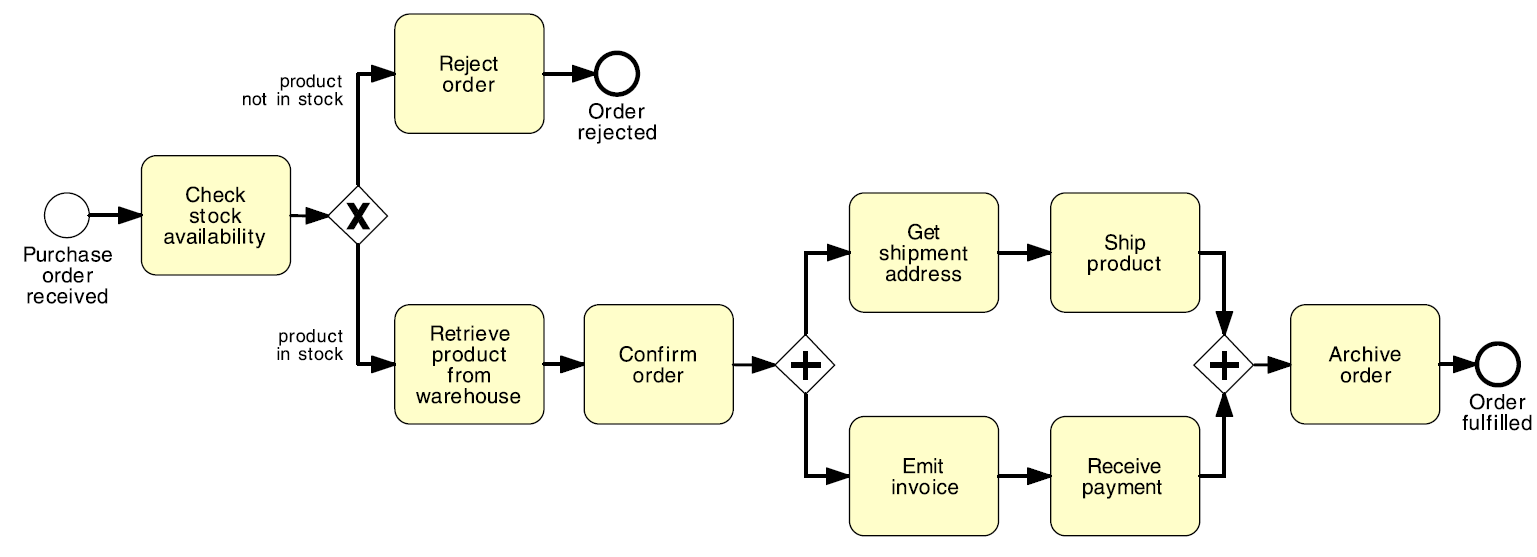
\includegraphics[width=\textwidth]{figures/bpmn.png}
    \caption[An example order fulfilment process in the Business Process Management Notation 2.0 ]{An example order fulfilment process in the Business Process Management Notation 2.0 {\cite{dumas2013fundamentals}} }
    \label{fig:bpmn}
\end{figure} 

% @article{dumas2013,
%   title={Fundamentals of business process management},
%   author={Dumas, Marlon},
%   year={2013}
% }

BPMS can interpret these process models and contains all kinds of functionality to deploy the described functionality of the process models in practice. For example, it can invoke financial systems to check whether the order is paid, notify users to pick certain items, communicate with customers and reorder new products. All this functionality is described in process models.

\subsection{Resource perspective} \label{section:introduction_resource_perspective}
The resource perspective consists of methods to manage the resources involved in the process executions. Resources can be either durable or non-durable. This thesis focusses on durable resources, i.e. resources that are claimed and released during the execution but are neither created nor destroyed before or after usage \cite{Huang2012,Huang2011a,Russell2004}. Examples of durable resources are employees, machines, books and cars. Examples of non-durable resources are software instances, raw materials and fuel.

Resources are the ones who perform the actual non-automated tasks and are therefore essential for the process execution. However, resources are not always available so the BPMS should plan the tasks according to a schedule. Furthermore, it is common that not all resources can perform all activities, thus the BPMS should also take this into account. Moreover, it is rather wasteful to randomly assign tasks to resources when a certain resource is already working on a large number of tasks, while the other resource has nothing to do. Finally, resources should also prioritize their tasks, because some tasks can have a higher priority than others and the resources only have a limited amount of time to perform a number of tasks. In order to take into account all these (and many more) problems, BPMS contain Work-allocation rules. The following sections discuss three types of resource work-allocation rules, namely: roles, resource allocation and resource prioritization.

\subsubsection{Roles}
Roles are part of Role-based access control (RBAC), which is a security policy dating back from 1996 \cite{rbac}. Today many organizations use RBAC to manage permissions within their organization \cite{rbac2,rbac}. In RBAC, each user has one or more role, whereas each role permits the access to one or more objects \cite{rbac2,rbac}. There are different kinds of permissions (e.g. read, write, own) and different kinds of objects (e.g. pictures, documents, databases) but for the scope of this paper, we only consider the permission to perform a certain activity. Whenever a user changes its position in the organization, its roles are changed. Similarly, whenever all users of a role (e.g. accountants) need permission to a new object, the role is simply changed. This is a major advantage over older security policies such as Discretionary Access Control (DAC) \cite{dac} and Mandatory Access Control (MAC) \cite{mac} where all permissions are stored on the user level so that for each user changes have to be made. 

Roles can be seen as a high-level work-allocation pattern in the context of BPM because it can determine which set of resources is allowed to perform a certain task. This narrows the search down for finding a resource to perform a certain task from the entire resource population to a set of resources. The next section describes how to further narrow down the search to an individual resource.

\subsubsection{Resource allocation}
Resource allocation rules or patterns define how to choose which resource should perform a certain task. There are two basic resource allocation pattern categories, namely: pull and push patterns \cite{hofstede2009modern, aalst2003workflow}. Pull patterns describe a situation where resources can decide which task they would like to execute and allocate the tasks to themselves. Contrary, push patterns describe a situation where the BPMS decides which resource should perform which tasks. Push patterns are much more complicated to implement because the pull patterns simply outsource the allocation to users whereas for push patterns the BPMS should perform the allocation automatically. Therefore, there are several elements of push patterns which each can help finding the most suitable resource for a given task as is discussed below. 

An important resource attribute is its availability, i.e. is the resource available? If so, what is its capacity? Is its capacity shared among other processes? How long is a resource available? The BPMS should, of course, only allocate tasks to resources which are available or becoming available in the near future, to prevent the situation that process instances keep waiting for resources which are simply not available. 

Another resource attribute is its preference or speciality, which describes what kind of tasks a resource prefers or is specialized in. This is important because specialized resources can better (e.g. higher quality/faster) perform certain activities than other resources. It can be the case that certain resources have more experience with handling certain tasks or simply like certain activities more. Note that a resource can also prefer certain case types (e.g. house loan request vs boat loan request or high-value loans vs low-value loans) instead of simply only certain activities.

Furthermore, another important resource attribute is its workload, i.e. the amount of  work allocated to a resource has. The workload should, of course, take into account the availability, but also the estimated task duration. The workload can be seen as a queue, where the tasks are waiting before the resource is available to perform the tasks. How resources handle such a queue is described in the next section. 

Finally, for compliance reasons, it might be the case that a previous resource allocation might limit the choice of resources in the future. For example, the 'four-eye' principle or 'dynamic separation of duty' pattern \cite{rbac} describes a situation where a resource might not be allowed to perform a task when it already performed another task for the same case. The four-eye principle can be used to prevent fraud. An example for such a situation is that a resource should not be able to create a large offer and also review the same offer because this offer should be reviewed by one of its peers. 

There are many attempts to combine the mentioned attributes into an optimal resource allocation model as is discussed in chapter \ref{chapter:background}. A rather naive method would be \textit{random allocation} or \textit{round robin} which both aim to provide each resource with an equal amount of tasks. An improvement could be to only look at workload, and allocate a task to the least-busiest resource, but this model still does not take into account availability and preference and will not motivate resources to finish their tasks as quickly as possible. 

\subsubsection{Resource Prioritization Rules}
Resource prioritization concerns only work list of a single resource and thus is relevant after tasks are allocated to a resource. The resource prioritization patterns describe how resources should handle the planning of its allocated tasks. There are various well-known resource prioritization policies, such as First-in-First-out (FiFo) and Last-in-Last-out (LiFo) \cite{hofstede2009modern}. Figure \ref{fig:fifolifo} illustrates FiFo and LiFo and shows that order of arrival is similar the execution order for FiFo. This is not the case for LiFo, where the latest arrived task is first performed. 

\begin{figure}[h]
	\centering
    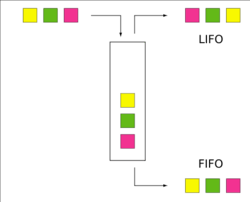
\includegraphics[]{figures/filo-lifo.png}
    \caption{A schematic illustration of FiFo and LiFo scheduling. The order of arrival is encoded into the worklist colours.}
    \label{fig:fifolifo}
\end{figure} 

\todo{Create better picture}

Furthermore, there are slightly more advanced policies such as Shortest Task in Queue and Shortest remaining case time. The Shortest Task in Queue prioritization policy simply estimates the duration of each event (e.g. by historical data or by heuristics) and the shortest task is chosen. The shortest remaining case policy estimates how long cases of the tasks in the worklist still need before they are finished, and picks the task with the shortest remaining case time. The latter policy aims to first finish all open cases before new cases are started. 

Finally, it is possible to extend each policy with priority, i.e. a different prioritization for high/low priority tasks. Each policy has its advantages and disadvantages and policies are seldom strictly followed. Each resource, role and department can have different prioritization rules.

\subsection{Application perspective}
The application perspective consists of a set of interoperability patterns which help the BPMS to communicate with external applications. The BPMS itself does not contain all functionality in an organization, it merely manages the process execution. This means that the BPMS is depended on many external applications. The BPMS can require external systems for the storage and retrieval of data (e.g. Customer Relationship Management (CRM) system for client data), but also outsource task execution to other systems (e.g. pay order task to the Enterprise Resource Planning (ERP) application) and can even be triggered by external systems (e.g. customer service desk received a call from a customer). Furthermore, communication can be synchronise and synchronize, and data routing can be dependent on various variables. There are also various methods for storing data such as repositories, relational databases, document-based databases and graph databases. 

The complete description of all these patterns is out-of-scope for this thesis. For more information, the reader is referred to \cite{russell2016workflow}.


\section{Process Mining} \label{sec:processmining}
Process Mining can be described as a set of quantitative analysis methods for business processes \cite{aalst2016process}. It is therefore often associated with the Business Process Management (BPM) domain \cite{aalst2013business} because of the focus on business processes, and the Data Mining domain \cite{kaufinann2006data} because of the focus on data and quantitative analysis methods. Process Mining is an emerging research field and gains many attention from the corporate and (semi-)governmental sectors \cite{aalst2011process,aalst2016process,aalst2012process}.

The basis of process mining is an Event Log \cite{aalst2016process}, which can be described as a dataset containing process related data. An Event Log contains at least a set of events, whereas each event describes change in time. Events have a time of occurrence, the type of task (activity) which is executed and the user who performed the event. Furthermore, the events are grouped in cases, whereas each case is a logical categorization of events, for example: each case describes a customer complaint handling, bank loan request or permit request. An Event log contains arbitrary many cases and each case can contain arbitrary many events.  

The three traditional pillars of process mining are: \textit{process discovery}, \textit{conformance checking} and \textit{process enhancement} and are all actively researched \cite{aalst2016process,aalst2011process}. \textit{Process discovery} focusses on describing the event log in terms of a process model. It aims to find the best possible process model for a given event log. \textit{Conformance checking} focusses on finding deviations of an event log to certain policies and is therefore mainly of interests for auditing purposes. Finally, \textit{process enhancement} aims to improve a discovered process model based on an event log by enriching the process model with additional or higher quality information.  

Furthermore, process mining has different perspectives \cite{aalst2016process}. Traditionally, the most important perspective is the \textit{control-flow} perspective, which describes the logical relations between activities and is often visualized in the form of a process model and is an integral part of the process discovery pillar \cite{discovery}. Another perspective which is often analysed is the \textit{case} perspective, which contains a collection of all events for each case. Furthermore, the \textit{organizational} perspective is also researched and aims to provide insights in the organizational hierarchy and rules such as identifying social networks \cite{van2007business,socialmining}. Moreover, the \textit{data} perspective contains additional optional data attributes and aims to find interesting correlations to improve process understanding or for the purpose of conformance checking \cite{DeLeoni2012,rogge2016log}. Finally, a well-studied BPM and process mining perspective is the \textit{time} or \textit{performance} perspective which describes the timing of events \cite{hornix2007performance,aalst2012replaying, aalst2009performancevis}. This perspective contains essential information for traditional business process improvements such as identifying bottlenecks and lowering throughput times.

One perspective which is missing and is often not considered explicitly is the \textit{resource} perspective \cite{Zhao2015}. The resource perspective contains information on which individual resource (e.g. employee, machine or system) performs which events. The resource perspective is somewhat related to the organizational and performance perspective. However, the former does not focus on individual resources and the latter tends to focus on the process as a whole and not on individual resources. This seems remarkable because resources seem to have a major impact on the process performance as they (i.e. employees) tend to be unpredictable, unreliable, error-prone and performing tasks with varying amounts of quality \cite{Pika2015}. Many BPM research acknowledges the fact that resources are an important factor, perhaps event one of the most important factors, of a business process \cite{baccarini2004management, Pika2015,thevendran2004perception}. 


\section{ProcessGold}
\todo{The introduction should contain a description of ProcessGold}


\section{Thesis description}
This section outlines the content of this thesis and is composed of a main research question and several supporting sub-research questions. The main research question is defined as:

\vspace{.5cm}
\textbf{RQ} How to analyse the impact of resources on cases and the impact of all cases on resources?
\newline


The question specifically focuses on the resource perspective. The resources perform the tasks of business processes and have therefore a significant impact on the process execution. Therefore, it is important to have a framework for analysing resources in a structured manner. The first step towards creating such a structured analyse method is to identify what is the current state-of-the-art in this area. The second step is to find relevant questions that need to be answered by the analysis method. Both steps are summarised in the first two sub-research questions, which are shown below. 

\begin{enumerate}
	\item[\textbf{RQ1}] What is the current state-of-the-art of resource-perspective analysis? 
    \item[\textbf{RQ2}] What are relevant resource-related questions and problems?
\end{enumerate}

\noindent
In order to answer RQ1, a literature study should be concocted to identify the latest developments in the resource-perspective analysis. Similarly, a literature study of the Business Process Management literature is also required in order to answer RQ2. Additionally, interviews with domain experts and consultants can also contribute to answering this research question. 

The structure of the rest of this document is as follows. Chapter \ref{chapter:background} aims to answer RQ1 by discussing the state-of-the-art literature on resource analysis. Chapter \ref{chapter:thesisoutline} then discusses relevant questions and problems for the resource perspective in order to answer RQ2. \todo{Add other chapters}





















\clearemptydoublepage

% \chapter{Preliminaries}\label{chapter:preliminaries}
% This template has been used to publish the thesis of Buijs~\cite{MScBuijs2010} and is originally used for the thesis of Nugteren~\cite{MScNugteren2010}. 

One of the best resources for \LaTeX basics, and advanced constructs, is the \LaTeX wikibook\footnote{To be found at~\url{http://en.wikibooks.org/wiki/LaTeX/}}. Of course colleagues and a good internet search using your favorite search engine can do wonders if you're stuck. 

\clearemptydoublepage

\chapter{Background Information}\label{chapter:background}
\label{section:resourceperspective} 
This chapter presents an overview of the state-of-the-art resource-perspective analysis in the context of process mining and aims to answer resource question RQ1. Moreover, this chapter also briefly reviews the state-of-the-art papers and contains explores various possibilities for further work. This state-of-the-art resource-perspective analysis aims to include previous research which meets the following selection criteria: the paper has as subject both \textit{process} or \textit{process mining} and \textit{resource}, whereas the latter can also be indicated as \textit{user}, \textit{organization}, \textit{human} or \textit{role}. The analysis, furthermore, used the following tooling to find relevant materials: \textit{WorldCat Discovery}, \textit{IEEE Xplore}, \textit{Springer Link} and \textit{Google Scholar}. Moreover, references in the found papers are also evaluated according to the selection criteria. 

As mentioned in the previous chapter, the resource perspective focuses on which individual resources perform which events. Furthermore, as also mentioned in previous chapter this thesis focuses on durable resources. Currently available research on the resource perspective also tends to focus on durable resources and can be categorized using the following groups: 

\begin{itemize}
\item General statistics of resources
\item Resource allocation rules and recommendation
\item Resource prioritization policies
\item Resource as queues
\item Conformance checking on resource perspective
\item Role Mining
\item Resource behaviour simulation 
\end{itemize} 

The following sections briefly summaries the available literature of these categories including a discussion of their results. However, simulating resource behaviour is out-of-scope for this thesis because this thesis focuses on analyzing behaviour observed in the past from event logs for which simulation is not a suitable technique. 

\section{General Statistics of Resources} \label{section:generalstatistics}
Several researchers created an approach to measure general statistics of resources. Pika et al. \cite{Pika2015,Pika2017} created a framework for analyzing and evaluating resource behaviour in the form as metrics such as productivity, skills, utilization, preferences, productivity and collaboration. All these measures, except collaboration, focus on an individual research and are defined for the case, activity and performance levels. The latter meaning that the metrics are defined on different granularity levels. Furthermore, the metrics are all visualized over time and changes are detected using a context-free outlier and 'change-point' detection algorithm. The metrics are implemented in an open-source proof-of-concept ProM plugin and is validated using a real dataset. 

Additionally, Huang et al. \cite{Huang2012} created a similar approach by measuring resource preference, availability, competence and cooperation. The metrics are essentially similar to \cite{Pika2015,Pika2017} but the implementation contains different visualization methods. Instead of visualizing the metrics over time, social networks are generated which can help identifying similar or related resources. Finally, \cite{Huang2012} creates a rather basic approach of recommending event scheduling based on the defined measures. This recommendation engine does, however, not take into account the current workload of resources, which seems an essential variable. The recommendation algorithm is implemented in a, rather limited, open-source ProM plugin.


\cite{Nakatumba2013} \todo{add Nakatumba}
The discussed papers contain valuable metrics, however, they do not elaborate on these metrics by, for example, correlating changes in these metrics with process outcome, quality or throughput time. Furthermore, the metrics and their changes over time are only measured, there is not yet invested any effort in finding the cause of sudden metric changes.  

\section{Resource Allocation Rules and Recommendation} \label{section:allocation}
This section contains the current research on Resource Allocation Rules (RAR), which can be described as rules or patterns which help to allocate events to the best available resource. Furthermore, this section contains various approaches to recommend the best resource for a given event. Huang et al. \cite{Huang2012} is already discussed in the previous section and contains a basic allocation recommendation algorithm based on the preference and competence of resources. 

Zhao et al. \cite{Zhao2015} created a more elaborate resource allocation model by relating resource allocation and process performance. The authors aim to minimize process throughput time in terms of resource preference, cost constraints and resource availability criteria. The latter meaning that the current workload of resources is taken into account, which is already a significant improvement over \cite{Huang2012}. However, the resource availability is also depended on the 'resource potential', which is a combination of the following variables: age, gender, family status and educational status. Defining the resource potential in this way is a questionable approach. The algorithm implementation is not public and the validation is based on an unspecified dataset.

Arias et al. \cite{arias2015framework} created a dynamic resource allocation framework which is based on resources capabilities, past performance, and resources workload. In practice, this means that the paper uses the following six dimensions: \textit{frequency} i.e. how many times a resource performed a similar activity, \textit{performance} i.e.the average execution time of the resource, \textit{quality} i.e. customer evaluation of past performance, \textit{cost} i.e. costs of execution the event, \textit{expertise} i.e. 'ability level' of the resource for a certain activity and finally, \textit{workload}, i.e. the current idle level of the resource. The six dimensions could be extended with other dimensions such as cooperation level as is already shown by \cite{Huang2012}. The work is implemented but not publicly available, and is validated using a non-public dataset. 

Liu et al. \cite{Liu2012} created an apriori-based algorithm for unsupervised Resource Allocation Rule mining. These rules are in the form of $activity \to resource$, meaning that for each activity a resource is recommended. Each 'rule' contains a support, confidence and lift metric, and the rule with the highest confidence (which meets a certain support and lift threshold) is chosen as the best recommendation. This method is rather naive as it does not take into account time perspective and the control-flow perspective, meaning that changes over time are not captured in this model and that activities which take place at different places in a process are also not taken into account. Furthermore, the resource workload and the data perspective are also not considered. Moreover, the algorithm is not publicly available but is validated on a public dataset. 

Huang et al.\cite{Huang2011} elaborated on this research by creating a more general unsupervised learning algorithm which takes also into account arbitrary data attributes. This is a significant improvement because other data attributes might contain valuable information and can potentially improve the resource allocation rule mining. The algorithms are discussed in great detail, however, the implementation is not public. The validation is limited to only a simple synthetic dataset. While the concepts of this research seem more promising as \cite{Liu2012}, performance issues might occur on large datasets because the algorithm seems computational expensive. Furthermore, resource workload, case attributes, data attributes of previous events and the time perspective are not taken into account because of the same performance issues. 

Finally, Huang et al. \cite{Huang2011a} created a more elaborate semi-supervised reinforcement-learning-based resource allocation recommendation engine. The algorithm is also discussed in great detail and a public ProM implementation is also available. The method is, however, only validated using a synthetic dataset and the method can only optimizer a single dimension (e.g. costs or throughput time). 

Most of the currently available research uses a rather basic machine learning approaches, while more elaborate machine learning techniques are already developed. These new techniques can help in three ways, namely: finding more advanced patterns, better filtering uninteresting rules and better performance. The latter is especially important because event logs can be enormous in size and can contain hundreds of data attributes. Simple naive data mining techniques cannot handle these quantities. Furthermore, the identified rules could be grouped and generalized such they become useful for end users \footnote{Note that the discussed approaches generate thousands of highly similar rules.}

\section{Resource Prioritization Policies} \label{section:prioritization}
Resource prioritization policies can be described as methods of how resources handle their own tasks on their worklist. Suriadi et al. \cite{Suriadi2015} investigated the resource prioritization policies by defining an approach of measuring which policies are followed. The authors focussed on FiFo, LiFo and prioritized FiFo. The latter being an extension of FiFo where a certain attribute is taken into account which denotes the priority level of an event. Their approach is to generate the worklists for all resources at all points in time and by simply walking through the log and assigning a penalty to each prioritization policy violation. The authors then visualize the penalty per resource, case or activity over time. Due to the nature of the penalty function, the algorithms do not find which prioritization policy is followed, but rather provide a relative scale on how much violations occur for each policy. It is not trivial to interpret this penalty value as it does not imply which prioritization policy is followed. Furthermore, there are more advanced prioritization policies which are not yet taken into account. Finally, many processes contain some kind of batch processing which interferes with the penalty score. The algorithms are implemented into an open-source ProM plugin and are validated using a synthetic and real dataset. 

There is no other research available in this field. However, the current work can easily be extended. For example, instead of just identifying which prioritization policies are followed, it might be interesting to measure the effects of such a prioritization policy on the event/process outcome, quality or performance. Furthermore, resources can be clustered based on their prioritization policies and changes in time can be detected and their cause and effect can be analysed. Sudden changes in prioritization policy might indicate changes in process definition or special periods such as holidays. 

\section{Resources as Queues} \label{section:queues}
Queueing theory is the mathematical study of waiting lines \cite{gross2008fundamentals, wolff1989stochastic}. The basic concept of queueing theory is that a durable resource needs to be shared among different users. The servers (resources) can only work simultaneously on a limited amount of tasks (often just a single task in the context of queueing theory), and thus a waiting line (or queue) of tasks appears. Queueing theory has a strong mathematical foundation and includes many prediction methods such as calculating the resource utilization or the average queue length. In the context of the resource perspective of process mining, it is possible to see resources as \textit{servers} and the worklist/backlog of allocated events as a queue. 

This is exactly what Senderovich et al. researched in \cite{Senderovich2014}. The authors created a method which is based on Queueing theory and using the available prediction methods of Queueing theory to predict delays in a process. The method is validated on a real dataset, however, the implementation is not publicly available. Furthermore, the method is limited to  homogeneous case types. The latter limitation is solved in a future work of the authors \cite{Senderovich2015b}, where the method can take into account different case types (such as customer types). This method outperforms the previous method. Both methods are described in great mathematical detail. However, just as the former method, there is also no implementation available for the latter method. 

Furthermore, Senderovich et al. the \cite{Senderovich2015a} also approached to join process mining techniques and queue mining techniques for performance analyzing by introducing Queue Enabling Colored Stochastic Petri Nets (QCSPN). This work is an initial step in closing the gap between these two techniques. Again no implementation is available, but the methods are validated on a real dataset. 

Because the absence of an open-source implementation, it is hard to compare the methods to other prediction approaches such as data mining algorithms. It would be interesting to compare different data mining algorithms against the queueing theory prediction on real data. Finally, the current work only focuses on predicting the case throughput time, but traditional queueing theory consists of much more predictions such as average workitems in queue and resource utilization rate. It would also be intersting to see how these predictions perform on real data.

\section{Conformance Checking on Resource Perspective}
Conformance checking traditionally focuses on the control-flow perspective and aims to find deviations from a policy in indivudal cases. Such a policy can be a predefined process structure, but also just a set of rules. Until recently, there was very little focus on the resource perspective as the only resource perspective specific conformance checking method was the 'four-eyed principle', where two events should not be executed by the same resource. 

De Leoni et al. \cite{DeLeoni2012} proposes a conformance checking approach which takes into account the resource perspective and can abstract from the data and control-flow perspectives. Traditional conformance checking algorithms first align the event log with the control flow, while this method concerns primarily about the resource perspective. Although this approach seems promising, it is only validated using a simple synthetic dataset. However, the implementation is available in an open-source ProM plugin. 

Mannhardt \cite{Mannhardt2018} created an extensive conformance checking framework which can balance the control-flow, data, resources, time perspectives. Furthermore, the author defined multi-perspective versions of traditional process mining metrics such as precision. The methods are validated using multiple real datasets in four case studies and the implementation is available as open-source ProM plugin. 

Because of the generalization of the previously discussed frameworks, most conformance checking problems can be solved by these frameworks. A possible further step could be to automatically identify the effects, or perhaps even causes, of the deviations. 

\section{Role Mining}\label{section:rolemining} \todo{add role clustering}
Role Mining emerged after the introduction of Role-based Access Control (RBAC) \cite{rbac2,rbac} and aims to group resource permissions in such a way that optimal roles can be constructed. RBAC is an access control approach which aims to manage resource permissions by defining resource roles. Each role contains a set of permissions on objects (e.g. files, processes, systems). Furthermore, users can be part of one or more roles. Before RBAC, organizations either used Discretionary Access Control (DAC) \cite{dac} or Mandatory Access Control (MAC) \cite{mac} which manages permissions on an individual resource basis. Because roles are more static over time than individual resources, the management of the security policy becomes less time-consuming \cite{rbac2,rbac}. In order to migrate from these old security policies to RBAC, roles should be defined. and thus \textit{role engineering} was created \cite{coyne1996role,roeckle2000role}. This is a set of techniques to define roles using a top-down approach, namely analyzing the organization and defining the roles based on domain knowledge. 

The top-down approach is time-consuming and rather error-prone, especially for large organizations with tens of thousands of employees and objects \cite{Kuhlmann2003}. Therefore, a bottom-up approach is created which analyzes all the permissions and tries to cluster the permissions in optimal roles without any domain knowledge using unsupervised machine learning algorithms. The input for the algorithm is a binary $User \; x \; Permission$ matrix, i.e. each user either has or does not have a certain permission. The output of the algorithm is two matrices, namely: a $User \; x\;  Role$ matrix and a $Role\;  x \; Permission$ matrix. The former matrix describes which roles the users have (N:M relation), and the latter matrix describes which permissions are each role has (also a N:M relation). The goal of the algorithm is to find clusters which are compatible with the old situation (i.e. no new permissions are allocated and no permissions are revoked) and to optimize the usability of roles (i.e. one could simply create a unique role for each user, but this is not against the principles of RBAC).

Kuhlmann et al. \cite{kuhlmann2003role} exactly followed this approach and used a clustering technique to identify the best roles. The techniques are evaluated on two non-public datasets using without quantitative metrics. Schlegelmilch et al. \cite{Schlegelmilch2005} followed another approach, namely by using subset enumeration on all permissions in order to find  all roles. The authors created two version of their algorithm, one which finds all roles but is rather inefficient, and a more efficient algorithm which has no guarantee that it founds all roles. The techniques are not evaluated in the paper, nevertheless, there is an open-source implementation available.

Zhang et al. \cite{zhang2007role} approached role mining as a graph optimization problem, where each user and permission are nodes and each edge represents an user owning a certain permission. The algorithm takes into account hierarchical roles and finds the optimal hierarchy based on the iterative merging of clustering. However, the algorithm is only evaluated on a small dataset and the implementation is not public ally available. 

These Role Mining are all based on the fact that all permissions are binary. Furthermore, the input of role mining is a matrix of $User \; x \; Permission$. This data is, however, not available in traditional process mining. The only related data which is available is the number of activities which resources perform over time. It is possible to convert this information to a binary $User \; x \; Permission$ table, but this would yield a lot of data loss (e.g. a resource which performs an activity 10,000 times is equal to a resource which performs the same activity a single time). It might be interesting to create a role mining algorithm which is tailored for a process mining scenario, in other words: it takes an event log as input instead of the $User \; x \; Permission$ matrix. 

\section{Conclusion}
The previous sections described the available state-of-the-art research on process mining and the resource perspective as is required for research question RQ1. For most categories, there is plenty of possible further work with the exception of conformance checking on resource perspective. In general, most work focus on identifying certain artifacts but do contain sufficient analysis to identify the (root)-cause of the artifact. Furthermore, the presentation of certain identified artifacts is suboptimal, therefore making it more challenging to use it in a business scenario instead of a research scenario. Finally, for role mining, there is no implementation which is tailored for a process mining setting.

These points can be used as starting point for defining resource-related research questions as is discussed in the next chapter. Each research question can be further decomposed in concrete problems which can be solved when the research question is answered. These problems can be identified and prioritized by performing structured interviews of domain experts.










\clearemptydoublepage


\chapter{Research Problem Definition}\label{chapter:thesisoutline}
This chapter elaborates on the previous chapter by describing relevant resource related problems, thus aiming to answer research question RQ2 and furthermore acting as a framework to structure the thesis. 

This chapter defines several sub-questions which each describe different relations between resources and cases. For each of the sub-questions, the goal is defined and the general problem is explained. Next, the evaluation for each sub-question is discussed and the high-level overview of possible techniques is given. 


The first sub-question aims to abstract from single resources by grouping them in roles. The next question focusses on finding resource and role bottlenecks which can be identified by studying their behaviour. Next, it is possible to analyse the common behaviour of the resources and roles by finding work-allocation patterns. These patterns can then be used to identify the deviating cases and hence it can be analysed whether the deviations have something in common using a root-cause analysis. Finally, it is important to take into account situations where insufficient information is available to perform the analysis.
 \todo{Add research questions about how to present the results to users in a intuitive way}

\section{Role Mining}
The goal of Role Mining is to identify the roles of resources based on event data. The resource roles can be used to abstract from individual resources because an event log can contain hundreds of resources and analyzing all resources on an individual level might not be feasible. A logical method for grouping resources are roles because many organization use roles to determine resource rights (see section \ref{section:rolemining}). 

This problem is different from the traditional role mining algorithms as described in section \ref{section:rolemining} because the input is now an event log instead of a set of permissions. In this setting, the exact permissions of roles are not of interest but rather the behaviour of the resources are of interests. The reason for this is because the roles are in this context not used for defining an access policy, but rather for analyzing the resource behaviour. The role mining should. therefore, identify roles based on the resource behaviour. Resource question RQ3.1 describes the identification of resource roles and  RQ3.2 elaborates on the identified roles by analyzing role behaviour. 

\begin{enumerate}
	\item[\textbf{RQ3.1}] Can roles be re-identified from event logs?
    \item[\textbf{RQ3.2}] Which activities are performed by which roles?
\end{enumerate}

\subsection{Evaluation}\label{section:role_mining_evaluation}
The output of the Role Mining is the identified roles for each resource. These results are evaluated using several methods. First of all, it is possible to simulate a synthetic process by using, for example, CPN Tools and define several resource roles which are each able to perform a set of activities. The process simulation tool should generate several event logs with various amounts of process instances (e.g. 100, 1,000, 10,000 and 100,000) which are loaded into the role mining algorithm. The results of the role mining can then be compared with the process definition. Furthermore, the event logs can be altered with certain noise levels (i.e. swap a certain percentage of a resource of an activity for another resource) and the results can again be compared in order to see how the algorithm performs in a more real-life setting. 

Furthermore, a more realistic setting would be to evaluate the clustering on a real-life log where the roles are known. Moreover, the clustering should be showcased on other real logs and, if available, the results can be discussed with a domain expert. 

\subsection{Technique}
Role Mining can be defined as an unsupervised machine learning problem because the roles should be predicted without the availability of a train set with 'true'-labels. More specifically, the problem relates to unsupervised clustering because the resources are clustered into roles. However, traditional clustering aims to find only a single cluster for each data point and can therefore not be used for this purpose because resources can have multiple roles. In the context of traditional clustering, a cluster would be a role or a set of roles and thus makes the results hard to interpret.

Furthermore, hierarchical clustering might be used because it generates hierarchical clusters, where each parent-cluster could mean that a resource contains the roles of the child-clusters. It is, however, challenging to find the right amount of cluster granularity when using hierarchical clustering and the hierarchy does not evaluate all role combination. Additionally, another clustering approach is Fuzzy Clustering which uses Fuzzy Logic. Each element is related to all clusters with a certain weight factor and can thus be part of multiple roles. This seems more suitable for role mining. The main challenge is to find the most optimal weight-threshold to convert the Fuzzy logic to role relationship logic. \todo{What about weighted graph clustering?}

By defining Role Mining as a clustering problem, it is possible to use the clustering metrics to evaluate the model. Examples of  unsupervised clustering metrics are: Root-mean-square standard deviation (RMSSTD) index, silhouette index, Davies-Bouldin, Calinski-Harabasz,Dunn index, R-squared index, Hubert-Levin (C-index), Krzanowski-Lai index, Hartigan index, Semi-partial R-squared (SPR) index, Distance between two clusters (CD) index, weighted inter-intra index, Homogeneity index and Separation index. A set of these metrics can be used to evaluate and compare the clustering models. Furthermore, another evaluation method is to divide the event log into a training and validation set to perform a cross-validation. 

% \noindent
% The evaluation is key for role mining, especially because role mining can be defined as an unsupervised learning problem and thus evaluation of the results is rather challenging. 

% \todo{Is there any other evaluation method which might be more meaningful for end-users?}

% Additionally, a more practical approach would be to test the clustering on a synthetic process log which is engineered in such a way that certain clusters are contained in the log. It is then possible to check whether the clustering approach can identify the clusters. 

% Finally, it is important to visualize the results. A visualization method is to plot the social graph by cluster. An extension would be to take into account the control-flow of cases, and to let the cases \textit{flow} between clusters.


\section{Bottlenecks}
The goal of the bottlenecks questions is to identify bottlenecks, analyse whether it changes over time and to find the root-cause of bottlenecks. Furthermore, this section elaborates on Role Mining because it uses the identified roles as input for the analysis. Moreover, the bottlenecks analysis elaborates on the general statistics of resources and resources as queues literature of section \ref{section:generalstatistics} and \ref{section:queues} because it builds on top of these methods.

In order to identify bottlenecks, it is essential to first estimate the utilization rate of resources (RQ4.1) because the utilization rate can be used to determine bottlenecks. Next, it is interesting to see whether there are any changes of the utilization over time, and what causes these changes (RQ4.2 and RQ4.2.1). Finally, it is key to identify the bottlenecks because the throughput of a process is limited by its bottlenecks (RQ4.3) and to find its root-causes (RQ4.3.1). 

\begin{enumerate}
\item[\textbf{RQ4.1}] How do we estimate the utilization of resources and roles?
\item[\textbf{RQ4.2}] Are there any significant changes in utilization of resources/roles?
  \begin{enumerate}
  \item[\textbf{RQ4.2.1}] If so, are there any predictors for the change? 
  \end{enumerate}
\item[\textbf{RQ4.3}] Which resources or roles act as a bottleneck in the process? 
  \begin{enumerate}
  \item[\textbf{RQ4.3.1}] If so, is it possible to find its root cause? \todo{remove this question? It is hard to validate. The output of 4.3 can be used as input for a root-cause analysis.}
  \end{enumerate}
\end{enumerate}

\subsection{Evaluation}
The output of RQ4.1 is a utilization rate for each resource on all points in time. In order to validate these utilization rates, a synthetic process can be simulated, similarly to the evaluation described in section \ref{section:role_mining_evaluation}. The simulation tool should output both an event log and the utilization rate of each resource over time. The event log can then act as input for the developed algorithm and the output can be compared with the output of the simulation tool. 

RQ4.2 aims to find changes in utilization rate, which can be validated similarly as RQ4.1 by building in certain change points in the synthetic process. Additionally, the change detection can be tested on real data where it is known that there is a process drift at a given point in time. Furthermore, for the purpose of evaluating RQ4.2.1, certain attributes can be injected into the process which are predictive of changes. 

Finally, RQ4.3 requires certain resources/roles which are a bottleneck in the process. Again, the simulated process model can incorporate this by creating a situation where the utilization rate of certain resources/roles is higher than one. The results of the bottleneck identification can then be compared with the actual bottlenecks. \todo{Remove 4.3.1 or add evaluation}

\subsection{Techniques}
Finding the utilization rate is dependent on two resource-independent attributes, namely: workload and availability. The utilization rate can be defined as the time that a resource is effectively working with respect to its availability. The time that a resource is working can be derived from an event log. The availability of resources, on the other hand, cannot directly be derived from the event log. It can be estimated from historical data how much time per period (e.g. week) a resource is available. This can then be used in combination with the workload to determine the utilization rate. The utilization rate identification is again an unsupervised learning problem. However, additional input can be given when the availability of resources is known. When this is not the case, the algorithm should estimate the availability. 

RQ4.2 aims at finding significant changes in a variable and can thus be defined as an unsupervised trend detection problem. An approach can be to detect trends in the data and see whether there are any significant changes in these trends over time. When there are significant trends in the data, RQ4.2.1 aims to find any predictors for the trends which can be approached by performing a regression analysis between case and event attributes against the trends. 

Finally, RQ4.3 aims to find which resources are the bottlenecks of the process and can thus also be defined as an unsupervised problem. The bottlenecks can be found because they limit the process throughput, i.e. the throughput of the bottlenecks is approximately equal to the complete process throughput. Furthermore, the throughput rate of the resources approach one, hence the workload keeps increasing over time. \todo{Remove 4.3.1 or add techniques}


% \noindent
% Question 4.1 can be validated by simulating a synthetic process and calculating the utilization rates of the resources at all times. This can then be compared to the chosen approach. Furthermore, many approaches to measure utilization of resources already exists in literature. Using an already proven metric can also contribute to the quality of the end-result. Question 4.2 can similarly be checked by simulating a synthetic process which contains changes in utilization rate over time. The predictors (Question 4.2.1) can again be evaluated using correlation errors. Finally, Question 4.3 can be evaluated in the same manner, but can also be evaluated by using real datasets where there is a known bottleneck. Additionally, the former results can also be showcased on real datasets. 

% Lastly, the visualization of the utilization rates can be projected on both the control-flow and the social graph. Furthermore, the changes in utilization rate can be plotted over time. 


\section{Work-allocation patterns}
The goal of the work-allocation patterns questions is to identify patterns in how tasks are allocated to resources as is shown in \ref{section:introduction_resource_perspective}. These work-allocation rules can be seen as more detailed patterns than the resource roles, which tend to focus on high-level inter-resource patterns, while work-allocation rules can be defined on individual resource level and even take into account other process perspectives. The questions in this section aim to create a general model of the current state-of-the-art techniques, which is presented in section \ref{section:allocation} and \ref{section:prioritization}. Furthermore, it extends the work by using the patterns as input for a root-cause analysis.

Research question RQ5.1 aims to find a set of work-allocation rules such as: \textbf{(a)} If multiple tasks are available, does a resource/role prefer a certain task?, \textbf{(b)} If there are multiple resources or roles are available for a certain task, is a certain resource/role picked more often? and \textbf{(c)} Which resource prioritization policies does a resource/role follow? RQ5.2 elaborates on RQ5.1 by analyzing whether there are any predictors for when certain work-allocation patterns are followed. \todo{What is the difference with deviations?}

\begin{enumerate}
\item[\textbf{RQ5.1}] Is it possible to detect work-allocation rules?
\item[\textbf{RQ5.2}] Do there exist any event or case attributes which can act as predictors for the work-allocation rules? 
\end{enumerate}

\subsection{Evaluation}
The output of RQ5.1 is a set of which resource patterns occur over time for certain resources or roles. The identified patterns can be validated by replaying the original event log and measuring how well the patterns describe the event log. Using this approach, the exact fitness, precision and generalization of the patterns can be calculated, which are defined as:

\begin{itemize}
\item \textbf{Fitness:} number of times which the pattern hold
\item \textbf{Precision:} number of times which the rule describes behaviour which does not occur in the event log
\item \textbf{Generalization:} relative score of how abstract the rule is 
\end{itemize}

The latter is important because a more high-level rule might be more useful as very detailed small rules. Note that a too general rule is penalized by the precision metric. Furthermore, it is again possible to evaluate the patterns on a synthetic process which is engineered to contain certain patterns. Moreover, it is possible to showcase the performance of the algorithm on real datasets. Finally, it is possible to compare the results with current approaches. 

Research question RQ5.2 outputs correlation factor for each attribute and can be evaluated by a different method, namely by using the correlation error of the event and case attributes. Furthermore, the correlation can be tested on a synthetic process and also public datasets. The findings of the latter can be confirmed by a domain expert. 

% Finally, there are various methods of visualizing the results, e.g.: highlighting the control-flow process model or social graph with the identified patterns. Moreover, the predictive capacity of the case attributes can be visualized for each work-allocation rule. 

\subsection{Techniques}
Because there are many different patterns, and some are better followed than others, RQ5.1 can be defined as an unsupervised ranking problem which aims to rank the work-allocation patterns on their relevancy or penalty. The problem is unsupervised because there is no training set available for the model to learn. In order to identify the patterns, an overall pattern model should be developed which can describe all patterns. Each pattern should then be defined in terms of this model and the event log should be mapped to the defined patterns. A way to approach this is to calculate alignments between the event log and patterns and then determine the evaluation metrics based on this alignment.  

Furthermore, RQ5.2 can be defined as a correlation problem, where each pattern can be correlated with all case and event attributes. These attributes might be able to predict which pattern is used. 


\section{Deviations}
The goal of the deviation questions is to identify when and why the work-allocation patterns and roles do not hold and thus elaborates on the previous two sections and the state-of-the-art techniques described in section \ref{section:allocation} and \ref{section:prioritization}. RQ6.1 aims to group deviations because just as with resources, it helps to abstract from individual deviations by grouping them. Furthermore, RQ6.2 aims to discover if there is a (set of) case and event attributes which can predict when deviations occur. The outcome of this question can be used for a 'root-cause analysis'.

\begin{enumerate}
\item[\textbf{RQ6.1}] Is it possible to group deviations from work-allocation rules? 
\item[\textbf{RQ6.2}] Are there any case attributes which can act as predictors for the deviations? 
\end{enumerate}

\subsection{Evaluation}
The output of RQ6.1 is grouped deviations. This can again be validated by extending the synthetic process model such that there are different reasons for a case to deviate from normal process execution. This process can be simulated and the event log can act as input for this algorithm. The identified grouped deviations can be compared to the actual deviation types. 

Research question RQ6.2 outputs correlation factor for each attribute and can be evaluated by a different method, namely by using the correlation error of the event and case attributes.

\subsection{Techniques}
Research Question RQ6.1 can be identified as an unsupervised clustering problem because it tries to cluster deviations into groups without learning from a training set. Because each deviation should be in exactly a single cluster, traditional cluster techniques can be used.  

Furthermore, R6.2 can be described as a correlation problem, where each deviation can be correlated with all case and event attributes. 


\section{Activity Life-cycle Transition}
The goal of the activity life-cycle transition question is to describe what to do when essential information, i.e. the start dates of events, is missing from the event log. All other components, except the role mining, are built on the assumption that this data is available. However, this is not the case in all situations and therefore it is essential to describe what to do when this information is unavailable. However, the current state-of-the-art research presented in section \ref{section:resourceperspective} does not take this issue into account. The final research question, RQ6, aims to find a solution for such a situation. 

\begin{enumerate}
\item[\textbf{RQ6}] What to do when no start activity life-cycle transitions are available?
\end{enumerate}

\subsection{Evaluation}
The result of activity life-cycle transition events is a start activity life-cycle transition for each event which does not have this information. An evaluation method is to strip the start activity information from a log and to estimate it. The average error between the estimations and the original data can be used to evaluate and compare different approaches. 

\subsection{Techniques}
The activity life-cycle transition question has to create information which is not available and can, therefore, be seen as an unsupervised prediction problem. Instead of just predicting the data, it is also possible to apply heuristics and use external data sources in order to estimate the start activity life-cycle transitions. 


\clearemptydoublepage

\chapter{Framework}\label{chapter:framework}
% This chapter discusses Role Mining in more detail. First the methodology of Role Mining is described in the first section. Next, the second section shows the results of Role Mining. Finally, the third section compares the results to the state-of-the-art role mining methods and section four shown the validation of the Role Mining approach. 

% \section{Methodology}
% This section describes the Role Mining approach. As previously mentioned in chapter 2, the goal of role mining is to re-identify RBAC roles from an event log. In order to do so, resources should be grouped based on their behaviour. In terms of process mining, the behaviour can be defined as the (relative) frequency that a resource performs  activities. In this case, the input for the role mining is thus simply an event log where each event contains the related resource.

This section discusses the chapter methodology of this thesis in the form of a framework. The main result of the thesis is a framework in which it is possible to estimate roles, identify resource bottlenecks and mine allocation patterns as discussed in the previous chapter. This framework describes how to approach these problems and furthermore an example implementation of each step is provided. The high-level overview of the framework is illustrated in Figure \ref{fig:framework}.


\begin{figure}[h]
  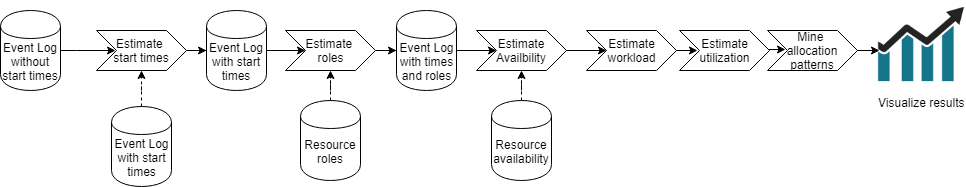
\includegraphics[width=\textwidth]{figures/methodology}
  \caption{High-level methodology overview}
  \label{fig:framework}
\end{figure}



Figure \ref{fig:framework} shows that for each of the three initial steps, it is possible to either provide input data or to estimate the data. In the latter case, the data is estimated and inserted into the event log as a log enhancement part. In the former case, the data is directly inserted as a log enhancement part. The availability estimation is dependent on earlier steps, i.e. roles and event log with start times, and this approach ensures that the analysis is always possible, even without the right data. \todo{Update model such that it is clear that steps can be skipped}

The initial input of the analysis is, just as with other process mining algorithms, an event log. More specially, an event log containing at least the following attributes: \textit{case id}, \textit{event id}, \textit{activity}, \textit{resource} and \textit{event end time}. Furthermore, the following attributes are optional: \textit{event start times}, \textit{other activity lifecycle transitions}, \textit{resource roles} and \textit{resource availability schedules}. Finally, all other case and event attributes, such as \textit{customer type}, \textit{case results} or \textit{organizational hierarchy}, can further enrich the analysis. For the scope of this framework, it is assumed that the event log is complete in the sense that it is represents the actual process execution. 

The next sections each discuss the exact inputs which are necessary for the analysis, the outputs which are generated by the step and which parameters and choices there are in the step. 


\section{Start time estimation} \todo{ToDo}
The first step of the framework is estimating event start times. This step can, of course, be skipped when the event log already contains event start times. 

% What are the inputs? 
% What are the outputs (results) 

% What are the intermediate steps, including choices/parameters. What is chosen and why, and what should be chosen by a domain expert. 

\section{Role Mining}
The next step of the framework is to estimate the roles of the resources including corresponding role hierarchy as defined in RBAC \cite{rbac2, rbac} as explained in section \ref{section:rolemining}. This step requires the activity executions per resource as input data and thus requires only an event log where each event is related to a resource. It is however not uncommon that a domain expert already knows the roles of the corresponding resources and it is also possible to use this information instead of estimating the roles. In this case, it may, furthermore, be interesting to see how the provided roles differ from the estimated roles (i.e., resource role conformance checking). 

Role Mining is, in this framework, defined as a clustering problem, where each cluster corresponds to a role and each data point to a resource. However, clustering itself is not sufficient for mining roles as it does not take into account the role hierarchy and the fact that resources can have multiple roles. The framework does include several heuristics to overcome this issue. 

The role mining outputs, for each resource, one or more roles and the role hierarchy of the event log. Similar to RBAC, employees can have multiple roles, while each role can have multiple related resources. Furthermore, a role can subsume other roles, thus resulting in a hierarchy of roles. Role mining step consists of seven steps. The sections below discuss each sub-step including an overview of all relevant parameters. 

\subsection{Generate input features}
The first step of role mining is to decide on the basis of which information the resources should be grouped into roles. RBAC roles are defined as a set of  permissions, whereas a permission $P$ can defined as pair of granted operations $OPS$ on certain objects $OBS$ \cite{rbac2, rbac}. In the context of role mining, there is only a single relevant permission, namely the right to execute a certain activity. Furthermore, the set of objects can simply be defined as all activities of a process. 

It makes sense to use this information directly as input features. Let $\#_{a}(e)$ be the activity of event $e$. The set of activities of a process can be mined and is defined as $acts(c) = \{\#_{a}(e) | e \in c\}$ and $acts(l) = \bigcup_{c \in l} acts(c)$ for case $c$ and event log $l$, respectively. Similarly, the set of resources can be defined as $res(c) = \{\#_{r}(e) | e \in c\}$ and $res(l) = \bigcup_{c \in l} res(c)$ for case $c$ and event log $l$.  

The actual input features can be defined as the relative frequency of activity executions per resources. Equation \ref{def:inputfeature} formalizes the relative activity frequency for a resource-activity pair, where $\#_{r}(e)$ equal to the related  related resource of event $e$. The relative activity frequency in Equation \ref{def:inputfeature} is defined as the number of times a resource performs an activity normalized by the resource's total activity executions. The normalization ensures that the sum of the relative activity frequencies of a resource is always equal to one. Without the normalization, the scores are dependent on how many events a resource performed in total, which should not influence the role definitions. 

\begin{equation}\label{def:inputfeature}
  \begin{array}{l}
    relative\_activity\_frequency(r,a) =  
    \cfrac{| \{e \in l | \; \#_{a}(e) = a \wedge \#_r(e)=r\}|}
    {| \{e \in l | \; \#_r(e)=r\}|}
  \end{array}
\end{equation}

Additionally, it is recommended to filter the relative activity frequency such that a score is only assigned when resource performed an activity a certain number of times. This prevents that resources which executed only a small amount of events distort the input features, e.g. when a resource only performs activity A, it gets a relative activity frequency of one while this can also be classified as noise. The filtered score is defined in Equation \ref{def:inputfeature_filtered} and only returns a score when the number of activity executions are higher than threshold $t$. The choice of $t$ is dependent on the event log, and can for example be defined as $(|\{e \in l\} \; / \; |res(l)|) \; / \; |acts(l)|)$, which is the activity frequency when a resource randomly performs activities. 


\begin{equation}\label{def:inputfeature_filtered}
  \begin{array}{l}
    rel\_act\_freq\_filtered(r, a, t) = 
    
    \begin{cases}
    	relative\_activity\_frequency(r,a), & \text{for } | \{e \in l | \; \#_r(e)=r\}| > t\\
        0 & \text{otherwise}
    \end{cases}
  \end{array}
\end{equation}

Moreover, the complete input feature is a $R  *  A$ matrix, where $R = res(l)$ and $A = acts(l)$, such that for each resource there is a relative activity frequency for all activities. Furthermore, it is possible to filter all resources which did not perform any tasks or almost any tasks. One can again define a certain threshold and check whether the sum of all activity executions are higher than the threshold. All resources which do not meet the threshold can be removed from the $R  *  A$ matrix.

\subsection{Pick Distance Metric}
The next step is to define a method which is able to check how (dis)similar resources are. These methods are known as distance function. Some well-known examples are euclidean distance, cosine distance and Manhattan distance. There is no distance function which works best on all event logs, thus the distance function should be chosen by a domain expert. 

The definition of these distance functions are shown below in Equation \ref{def:distance_euclidean}, \ref{def:distance_cosine} and \ref{def:distance_manhatten}, where $\mathbf{p}$ and $\mathbf{q}$ are two vectors representing resources, where each element in the vectors correspond with a relative activity frequency: $\mathbf{p}=(p_1,p_2,\dots,p_{|acts(l)|})\text{ and }\mathbf{q}=(q_1,q_2,\dots,q_{|acts(l)|})$.

\begin{equation}\label{def:distance_euclidean}
  \begin{array}{l}
    euclidean\_distance(\mathbf{p},\mathbf{q}) = \sqrt{ \sum_{i=0}^{|acts(l)|}(p_i- q_i)^2}
  \end{array}
\end{equation}


\begin{equation}\label{def:distance_cosine}
  \begin{array}{l}
    cosine\_distance(\mathbf{p},\mathbf{q}) = \frac{ \sum\limits_{i=0}^{|acts(l)|}{p_i  q_i} }{ \sqrt{\sum\limits_{i=0}^{|acts(l)|}{p_i^2}} \sqrt{\sum\limits_{i=0}^{|acts(l)|}{q_i^2}} }
  \end{array}
\end{equation}


\begin{equation}\label{def:distance_manhatten}
  \begin{array}{l}
    manhatten\_distance(\mathbf{p},\mathbf{q}) = \sum_{i=0}^{|acts(l)|} |p_i-q_i|
  \end{array}
\end{equation}

\noindent
The distance functions each work best in certain scenarios. The overview below discusses when the effect of the distance functions and in which situations they generally perform best in the context of role mining. Manhatten distance fits the data best because it evaluates the features completely independent and thus do not assume any relation between the features, contrary to euclidean and cosine distance. 

%However, Manhatten does not perform in all situations best. 

\begin{itemize}
\item \textbf{Euclidean} calculates the shortest distance between two points but is  sensitive to noise. It therefore performs best when there are many resources but not much noise in activities. 
\item \textbf{Cosine} calculates the angle between two vectors but ignores the magnitude of the vector. Therefore, it generally generates less roles and looks more at which relative activity frequencies are positive rather than the difference in scores. It is thus effective in situations where there are many activities and resources and is less sensitive to noise.
\item \textbf{Manhatten} sums the difference between all relative activity scores of resources and therefore is sensitive to small differences in the scores. This results generally in more roles and a more extensive role hierarchy. This distance function is most usable in cases where there are many resources with low number of activities.   
\end{itemize}

\subsection{Additional Preprocessing steps}
It is, furthermore, possible to include other common clustering preprocessing steps such as removal of uncommon activities and feature-wise normalization. This may be valuable in certain situations, but in general both preprocessing steps seem to have a negative effect on the results. The filtering of uncommon activities removes information from the input vectors. The fact that certain resources did not execute certain tasks is also valuable information. 

Furthermore, the feature-wise normalization also seems to impact the output quality in a negative way. Feature-wise normalization ensures that averages and variances within features become equal which has the effect that non-common activities become more important. This effect is clearly shown in Table \ref{table:input} and \ref{table:input_normalized} where Table \ref{table:input_normalized} contains the normalized features of Table \ref{table:input}. In this example, \textit{Activity B} is generally less common in the dataset, but the normalization causes a small difference in relative activity frequency score of \textit{Activity B} is seen as a large change. 

The normalization might be useful for situations where each activity is equally important. However, in most situations there are activities which are more prominent than other activities and thus the normalization might create a distorted view on the dataset. 

\begin{table}
  \parbox{.45\linewidth}{
    \centering
    \begin{tabular}{cccc}
    \hline
    Resource& Activity A & Activity B & ... \\
    \hline
	User\_1 & 0.3 & 0.1 & ... \\
	User\_2 & 0.8 & 0.2 & ... \\
	User\_3 & 0.6 & 0.1 & ... \\
    \hline
    \end{tabular}
    \caption{Example relative activity frequencies input vector}
    \label{table:input}
  }
\hfill
  \parbox{.45\linewidth}{
    \centering
    \begin{tabular}{cccc}
    \hline
    Resource& Activity A & Activity B & ... \\
    \hline
	User\_1 & 0 & 0 & ...\\
	User\_2 & 1 & 1 & ...\\
	User\_3 & 0.5 & 0 & ...\\
    \hline
  \end{tabular}
  \caption{Example input vector normalized with min-max normalization}
  \label{table:input_normalized}
}
\end{table}

Finally, when there are hundreds or even thousands of different activities, or performance is essential, it is also possible to consider a form of dimensionality reduction such as Principle Component Analysis (PCA). In general, dimensionality reduction reduces the time required for clustering but reduces the quality of the clustering. However, when the dataset contains a lot of noise, it may actually yield positive results. When applying dimensionality reduction, it is more challenging to interpret the results, i.e. see why certain resources are clustered together. 

\subsection{Clustering Algorithms}
The next step is to find the best clustering algorithm. There are seven different types of clustering algorithms and the overview below summarises the types and discusses their usefulness for role mining. \todo{sources}

\begin{itemize}
\item \textbf{Centroid-based clustering} aims to optimize the cluster centroid locations by iteratively moving the centroids such that the distance between each cluster and related data point is minimized. The algorithm requires the number of clusters as input which is most of the cases unknown.  
\item \textbf{Fuzzy clustering} is similar to centroid-based clustering but does not limit data points to a single cluster. In practise, this means that a resource can have a relation with multiple clusters, which is also the case with roles. This approach  requires, besides the number of clusters, a 'de-fuzzyfier' which converts the fuzzy relationships to role participation relations. The de-fuzzifier is sensitive to noise and therefore hard to optimize.  
\item \textbf{Agglomerative clustering} initially considers all data points as clusters and merges the two most-similar clustering until there is only a single cluster. The challenge of this approach is to find the best point to stop merging clusters. The advantage of this approach is that it naturally contains a cluster hierarchy which can be used as role hierarchy. However, it does not evaluate all cluster combinations, rather the local best solution which might not be the optimum solution. 
\item \textbf{Graph-based clustering} considers the clustering as a graph optimization problem and tries to find optimal sub-graphs, i.e. clusters, by iteratively cutting the graph in two sub-graphs. This approach also requires the number of clusters as input. Furthermore, this approach does not scale well with the number of clusters and can therefore not be used with large datasets. 
\item \textbf{Density-based clustering} iteratively finds neighbouring data points by checking whether there are any points within a certain range of cluster edges. This approach clusters points based on how similar they are to points in the cluster. This means in practise that not all resources in a clusters should behave as the cluster average, but rather comparable resources are grouped together based on their similarity with the edges of the clusters. The clustering algorithms requires the maximum range parameter which one point can be apart of a cluster (epsilon) and the minimum points per cluster.  
\item \textbf{Distribution-based clustering} This clustering approach does not scale well and can therefore not be used with large datasets. \todo{add description}
\item \textbf{Apriori Rule Mining} approaches to find 'rules' which meet a certain support and confidence threshold. Each rule relates employees to a set of activities. The approach keeps trying to find more complex rules based on the simple rules which meet the threshold, therefore yielding a tree-hierarchy between rules. This approach is, however, very sensitive to noise and generates already thousands of rules for relative small event logs. Furthermore, this approach is also computational expensive and does, therefore, not scale well. 
\end{itemize}

\noindent
The graph-based, distribution-based clustering and apriori rule mining approaches do not scale well with the number of data points and number of clusters and are therefore not usable in practise. Additionally, Fuzzy clustering performs poorly when there is a low amount of noise and therefore is also not usable in practise.

Density-based clustering fits the problem best because it aims to find similar resources based on their distances with their most-similar colleagues and is therefore better in handling slight variations in roles. Centroid-based clustering might be useful when there is low variation between employees, which occurs for example if there are not many activities. Finally, Agglomerative clustering may be useful when there is a lot of variation between clusters. 

Instead of choosing a clustering algorithm beforehand, the most usable algorithms (Density-based, Centroid-based and Agglomerative clustering) can be considered at the same time. The results of each algorithm can be compared and the best can be chosen by a domain expert.  

\subsection{Hyperparameter optimization}
The next step is to optimize the parameters of the chosen algorithms, which includes two important artifices, namely: an evaluation metric and the parameters of the clustering algorithms. When the right evaluation metric is chosen, it is possible to perform a Grid-search approach, i.e. testing each combination of algorithms and possible parameter combination. Other hyper-parameter tuning approaches such as Random Search, Bayesian optimization or Evolutionary optimization can also be used for performance reasons, but this only becomes relevant for very large event logs (e.g. thousands of resources and activities). Gradient-based optimization For performance reasons, the maximum number of iterations for the clustering algorithms can be limited. 

\subsubsection{Evaluation Metric}
Role Mining is defined as an unsupervised clustering problem, and therefore it is not possible to evaluate the results with the absolute truth as this information is unavailable. There are, however, other evaluation metrics for unsupervised clustering which are categorized as internal performance metrics which aim to evaluate goodness of a clustering structure without external information \cite{thalamuthu2006evaluation, dudoit2002prediction}. A well-known example of such a metric is the Silhouette index \cite{rousseeuw1987silhouettes}, which aims to measure how well data points belong in a cluster \cite{rousseeuw1987silhouettes}.

Other internal performance metrics include Davies–-Bouldin index, Dunn index, Calinski-Harabasz, Hubert-Levin (C-index) and Krzanowski-Lai index. Most of these metrics have either a positive or negative trend over the number of clusters, which make them challenging to use for hyperparameter optimization. This is not the case for Silhouette index, Dunn index and Davies-Building index and therefore these metrics are considered in the hyperparamter optimization. \todo{sources}


\subsubsection{Parameters}
Clustering algorithms have different parameters, and therefore the parameter optimization is different for each set of clustering algorithms. DBSCAN has two attributes, namely: the minimum data points in a cluster and the maximum distance between a data point and a cluster edge (epsilon). The former is relative simple as RBAC supports the fact that there is only a single resource related to a role as is discussed in section \ref{section:rolemining}. It therefore does not make sense to choose a higher value. 

However, the epsilon value is more challenging to optimize as it depends on the input features. It is, however, possible to reason about the maximum distance of a dataset, namely: each resource has $|acts(L)|$ number of relative activity frequency scores which range from zero to one. The maximum possible distance in the dataset is thus simply the number of activities. A possible improvement would be to calculate the maximum distance between resources in the event log by taking the maximum value of the distance matrix. It is then possible to try different epsilon values between zero and this maximum and to pick the epsilon with the best performance. 

The centroid-based and agglomerative clustering approaches both only have a single parameter, namely: the amount of clusters (k). It can be optimized is a similar way as the epsilon parameter by checking which k-value performs best. The maximum possible k-value is $|res(l)|$ and the minimum value is two. It is possible to simply evaluate all possible k-values in this interval. However, for datasets with many resources, it is possible to set a maximum to the amount of clusters, e.g.  $|res(l)| / 2$ which only evaluates situations where roles contains, on average, two resources (which is reasonable when considering that RBAC tries to maximize the amount of resources per role \cite{rbac2}).  

\subsection{Prediction}
Based on the output of the hyperparameter optimization, an algorithm with corresponding parameters is chosen. The clustering process is than repeated with a higher number of maximum iterations resulting in a $role(r)$ for each resource $r$. Let $Rs$ be defined as $Rs \;=\; \{role(r) \; | \; r \in res(l)  \}$. 

\subsection{Post-process and decompose roles}
The final step is the post-processing of the clusters into roles. The first step is to place all non-active resources which were removed from the dataset in a new "non-active" cluster. 

The following step is specific to DBSCAN, which places certain resources into an outlier cluster. These resources are not related to each other and therefore the resources should be placed each in their own cluster. 

Next, the clusters should be decomposed into roles by creating a role hierarchy. Each cluster is considered to represent either a single role or a set of roles. In order to find the role hierarchy, the roles are compared with each other. The first step to do so, is to calculate the average relative activity frequency for each role. Next, a single role (source role) is picked and compared to all other roles (target roles). If all activities of a target role, which have a higher average relative activity frequency than threshold $1/|acts(L)|$ (the score which is obtained when randomly performing activities), are also performed by the source role, the target role is considered to be a child-role of the source role. Equation \ref{def:sub_role} formally defines the sub-role relation between role ${r1}$ and role ${r2}$, given threshold $t$ and $r_i$ being defined as the $i^{th}$ average relative activity frequency of role $r$. Equation \ref{def:sub_roles} iterates over all roles ${Rs}$ to find all sub-roles of role ${r1}$.

\begin{equation}\label{def:sub_role}
  \begin{array}{l}
    is\_sub\_role({r1},{r2}, t) = \forall_{i=0}^{|acts(l))|}  \; {r1}_i > t \Rightarrow {r2}_i > t
  \end{array}
\end{equation}

\begin{equation}\label{def:sub_roles}
  \begin{array}{l}
    sub\_roles({r1},{Rs}, t) = \{r \in Rs \; | \;is\_sub\_role({r1}, {r})\}
  \end{array}
\end{equation}

\begin{table}[h]
  \parbox{.45\linewidth}{
    \centering
    \begin{tabular}{cccccc}
    \hline
    Resource& A & B & C & D & Role\\
    \hline
	User\_1 & 0.4 & 0 & 0.4 & 0.2 & 1 \\
	User\_2 & 0.9 & 0.05 & 0.0 & 0.05  & 2  \\
	User\_3 & 0.2 & 0 & 0.4 & 0.4 & 1 \\
    User\_4 & 0.3 & 0.15 & 0.15 & 0.4 & 3 \\
	\hline
    \end{tabular}
    \caption{Example role clustering results}
    \label{table:role_avg}
  }
\hfill
  \parbox{.45\linewidth}{
    \centering
    \begin{tabular}{ccccc}
    \hline
    Role& A & B & C & D\\
    \hline
	1 & 0.3 & 0 & 0.4 & 0.3 \\
	2 & 0.9 & \sout{0.05} & 0 & \sout{0.05}\\
	3 & 0.3 & \sout{0.15} & \sout{0.15} & 0.4\\
    \hline
  \end{tabular}
  \caption{Role averages with filtered scores, threshold: $1/|acts(L)|=0.2$}
  \label{table:role_avg_filtered}
}
\end{table}

Table \ref{table:role_avg} and \ref{table:role_avg_filtered} illustrate this process, where Table \ref{table:role_avg} contains the relative frequency scores for each resource including the predicted role and Table \ref{table:role_avg_filtered} contains the filtered role averages. In this example, role 2 will be classified as sub-role of both role 1 and role 3 because all the roles have a higher average relative activity frequency than role 2 and role 2 does not perform any other tasks than role 1 and 3 which meet the threshold. Furthermore, role 1 also subsumes role 3, as it performs all activities as role 3. The role hierarchy is thus defined as $\{sub\_roles({r1}, t)=\{{r2},{r3}\}, sub\_roles({r2}, t)=\emptyset, sub\_roles({r3}, t)=\{{r2}\}$ for $t = \dfrac{1}{|acts(L)|}=0.2 \}$ as results of Equation \ref{def:sub_roles_hierachy}.

\begin{equation}\label{def:sub_roles_hierachy}
  \begin{array}{l}
    sub\_role\_hierachy(t) = \{sub\_roles(r, t) \; |\; r \in Rs\}
  \end{array}
\end{equation} 

\todo{Add dashboard?}

\section{Availability}
The next step of the framework uses the (estimated) roles and start times to estimate the availability of each resource and each role. It is again possible that the domain expert already has this information and therefore this step might be skipped. In this case, it would be interesting to compare the provided availability with the output of this analysis. The availability analysis has significantly less parameters and choices than role mining.

The availability estimation outputs the times when a resource is generally available in two granularities, namely: the weeks a resource is available and the general work-schedule per weekday. The work-schedule contains for each weekday the half-hour timeslots that a resource is generally available. The reason for the choice of these two granularities is that weeks and workdays are both logical ways to divide a resource's time. The following section discuss how these two availability granularities are calculated.  

\subsection{Available weeks}
The first step of the availability analysis is to check which weeks resources are active. This is important because certain resources may start or stop working on the process during duration of the event log. Furthermore, resources can go on holidays or take time off, which would distort the analysis when is not taken into account. First, the time range of the event log is defined as $weeks(l)=\{ week(\#_{te}(e)) \; | \; e \in l \}$ where $week(\#_{te}(e))$ is the ISO8601 week-number \cite{iso8601} of $\#_{te}(e)$, i.e. the completion time of the event. 

\begin{equation}\label{def:events_per_week}
  \begin{array}{l}
    events\_in\_week(r, week) = \{ e \; | \; e \in l \wedge week(\#_{te}(e)) = week \wedge \#_{r}(e) = r \; \wedge \neg \; \#_{a}(e)\}
  \end{array}
\end{equation}

\begin{equation}\label{def:automated_events}
  \begin{array}{l}
    \#_{a}(e) = \#_{te}(e) - \#_{ts}(e) = 0
  \end{array}
\end{equation}

Next, Equation \ref{def:events_per_week} finds the executed events per week per resource, where $\#_{a}(e)$ is true when the event is classified as an automated event and false otherwise. The definition of automated events can differ between event logs but can be described as system events which are automatically performed by the system or automatically triggered when resources perform certain actions. It is important to filter out the automated events because they are not performed by the resource but rather by the system and therefore do not contain any information regarding the availability of this resource. A method to identify automated events can be found in Equation \ref{def:automated_events}, which simply checks whether the throughput time of an event is equal to zero. 

\begin{equation}\label{def:events_per_week_avg}
  \begin{array}{l}
    avg\_events\_in\_week(r) = avg(w  \in weeks \; | \; weeks_{P^{95}} > events\_in\_week(r, w) > weeks_{P^{5}})
  \end{array}
\end{equation}

\begin{equation}\label{def:active_week}
  \begin{array}{l}
    is\_active\_week(r, week) = \dfrac{avg\_events\_in\_week(r)}{5} < events\_in\_week(r, week)
  \end{array}
\end{equation}

Figure \ref{fig:available_weeks} uses the equations by visualizing the size of the $events\_in\_week$ for all weeks of a single resource where each bar represents a week and the height of the bar represents the number of events executed in this week. Furthermore, the Figure shows a black line which represented the average number of events per week when excluding the top and bottom five percentile of weeks as is defined in Equation \ref{def:events_per_week_avg}. The top and bottom percentiles ($weeks_{P^{95}}$ and $weeks_{P^{5}}$) are removed to prevent outlier weeks from having a large impact on the averages.

Moreover, the bars are coloured red when the weeks do not meet threshold $t$ and coloured green otherwise. The threshold $t$ can again differ between event logs and should be defined by a domain expert, but a method to determine it is to divide the average executed events per week by five as is shown in Equation \ref{def:active_week}. This would imply that if a resource does the same amount of work in a week what it normally does in a single workday (provided that a resource works five workdays a week), it is considered as inactive that week. 

\begin{figure}[h]
	\centering
    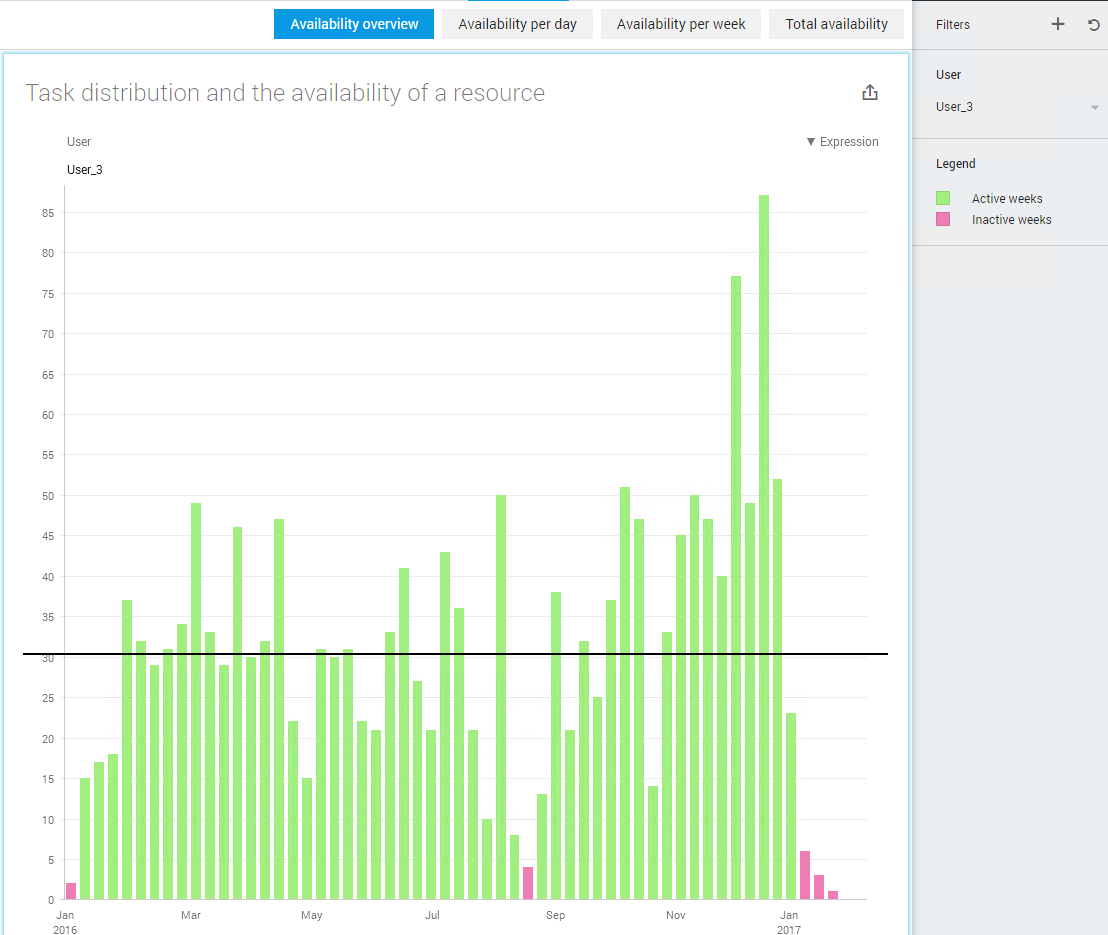
\includegraphics[width=\textwidth]{figures/available_weeks}
    \caption{Events executed per week for resource \textit{User\_5} of the BPIC2017 challenge including the average events per week.}
    \label{fig:available_weeks}
\end{figure}

\subsection{Available timeslots}
This section elaborates on the previous section by finding the availability of resources in preciser time periods of thirty minutes. For each weekday, forty-eight thirty-minutes periods are defined which totals 336 timeslots. Let $ts$ be the set of all timeslots for a week. For each timeslot and for each user the events are counted independent of the weeks. The timeslots are defined per weekday because it is assumed that resources may act differently depending on the weekday. The events per timeslots are only dependent on the available weeks, as only the active weeks are taken into account as is shown in Equation \ref{def:events_per_timeslot}. Similar to the previous section, it is possible to define a threshold for each timeslot to determine when a resource is generally available. 

\begin{equation}\label{def:events_per_timeslot}
  \begin{split}
    events\_in\_timeslot(r, timeslot) = \{ e \; | \; e \in l \wedge is\_active\_week(week(\#_{te}(e))) \; \wedge & \\
    \#_{te}(e) \in timeslot \wedge \#_{r}(e) = r \; \wedge \neg \; \#_{a}(e)\} & 
    \end{split}
\end{equation}


\begin{figure}[h]
	\centering
    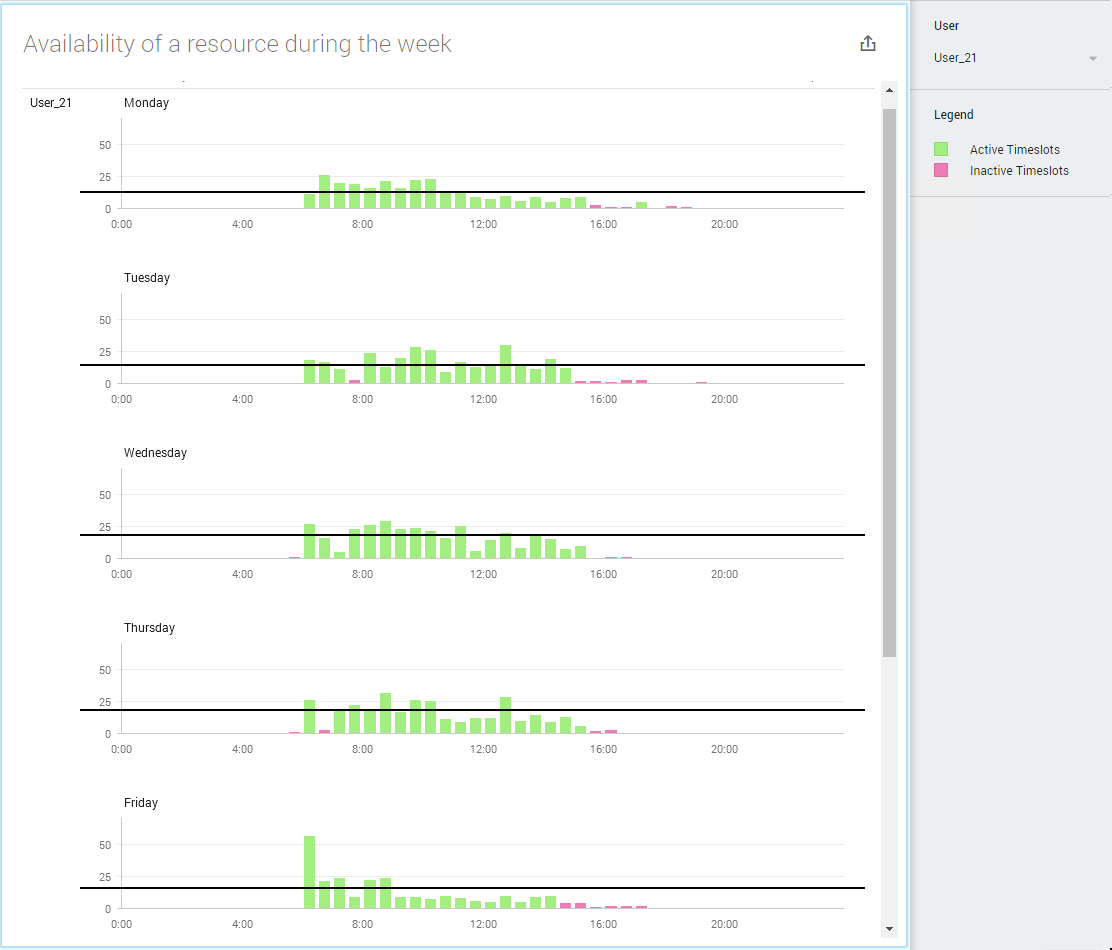
\includegraphics[width=\textwidth]{figures/available_timeslots}
    \caption{Events executed per timeslot for resource \textit{User\_21} of the BPIC2015 challenge including the average events per week.}
    \label{fig:available_timeslots}
\end{figure}

Figure \ref{fig:available_timeslots} illustrates the events per timeslot for resource \textit{User\_21} of the BPIC2017 event log. The Figure shows per weekday the events per timeslot and shows a clear pattern that the resource starts at 6:00 each morning and works until approximately 15:30. However, on Saturday and Sunday, \textit{User\_21} does not seem to work which is rather common in a forty hour work-week. Moreover, the resource seems to leave an hour earlier on Friday. Furthermore, resources may work only part-time and therefore not available on multiple other weekdays. This supports the assumption that resources might have different behaviour on each weekday. 

\begin{equation}\label{def:events_per_timeslot_avg}
  \begin{split}
    avg\_events\_of\_weekday(r, wd) = avg(\{t \in ts \; | \; weekday(t) = wd \; \wedge & \\ 
    ts_{P^{95}} > events\_in\_timeslot(r, t) > ts_{P^{5}} & \})
  \end{split}
\end{equation}

\begin{equation}\label{def:active_timeslot}
  \begin{array}{l}
    is\_active\_timeslot(r, t) = \dfrac{events\_in\_timeslot(r,t)}{5} < avg\_events\_of\_weekday(r, weekday(t))
  \end{array}
\end{equation}

Moreover, the Figure contains green and red colouring which have similar meaning as in Figure \ref{fig:available_weeks}, it indicates whether the timeslots meets a certain threshold. The threshold is defined in Equation \ref{def:active_timeslot} which uses Equation \ref{def:events_per_timeslot_avg}. The latter equation calculates the average events in a certain timeslot and is specific for each weekday $wd$, because it is assumed that resources might have different behaviour dependent on the weekday. Finally, the total available time per resource for the event log can calculated by simply multiplying the active timeslots with the active weeks. 

\section{Workload}
This section elaborates on the availability information by calculating the workload per available timeslot. The workload estimation uses the event start and end times as input and checks at each point of time how 'busy' a resource is. When projecting the workload onto the availability, it is possible to calculate the utilization rate of resources. It is possible to provide the workload and utilization step by manually providing the information. However, it seems rather unlikely that this information is available as it is rather detailed.  

\begin{equation}\label{def:workload_time}
  \begin{array}{l}
    workload(r,t) =  
    | \{e \in l | \; \#_{ts}(e)  \leq t \leq \#_{te}(e) \wedge \#_r(e)=r \; \wedge \neg \; \#_{a}(e)\}| \; 
  \end{array}
\end{equation}

The definition of workload is the amount of events which have started, but have not ended at a certain point of time for a certain resource as can be seen in Equation \ref{def:workload_time}. Again, the automated events are filtered because the resource itself does not perform these events. Moreover, it is possible to calculate the workload in a period of time. It is not possible to simply iterate over all points in time and calculate the workload at all points because time is a continuous value. Furthermore, this would not be an efficient method.   

\begin{figure}[h]
	\centering
    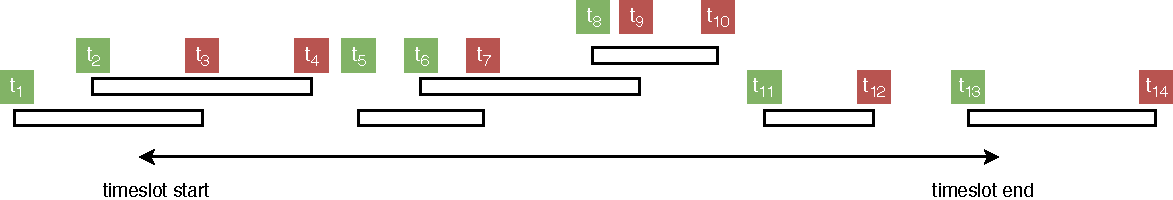
\includegraphics[width=\textwidth]{figures/workload_period}
    \caption{Workload during a time period where green points in time indicate a positive workload delta, and red points in time indicate a negative workload delta}
    \label{fig:workload_period}
\end{figure}

Figure \ref{fig:workload_period} illustrates an alternative method for calculating the workload during a time period. The first step is to filter all events which intersect with the time period, i.e.: $events = \{e \in l | \; \#_{ts}(e) \leq t_e \wedge t_s \leq \#_{te}(e) \; \wedge \#_{r}(e) = r \}$ for resource $r$ and time period $t$ where $t_s$ and $t_e$ denote the start and end times of the period, respectively. Next, it is possible to iterate over the chronological set of start and end times which are denoted in Figure \ref{fig:workload_period} as $t_i$. The workload is static except when an event starts or completes, where the workload is increase or decreased with one, respectively. 

\begin{figure}[h]
	\centering
    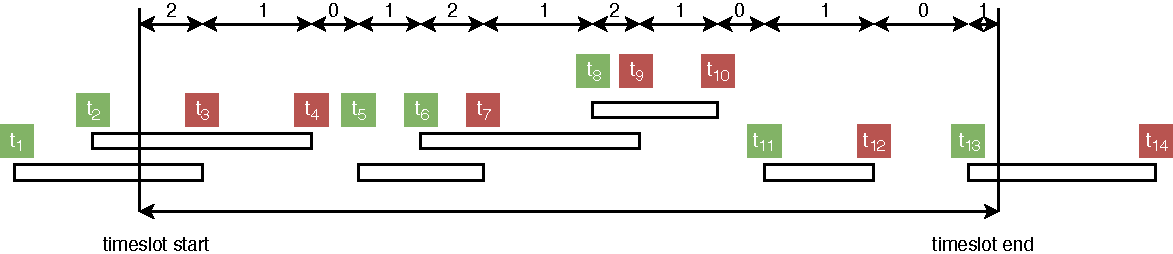
\includegraphics[width=\textwidth]{figures/workload_period_avg}
    \caption{Average workload during a time period where the top numbers indicate the workload for sub-periods of time}
    \label{fig:workload_period_avg}
\end{figure}

This method can be used to calculate the average workload during a time period by slightly extending it. The timeslot start $t_s$ and end $t_e$ should be added to the set of start and end times $t$, but should not decrease nor decrease the workload value. However, the algorithm should only take into account the time between these points for calculating the average workload. The algorithm iterates over this set of times and save the latest point in time which changes the workload as $t_{saved}$. Every time the workload changes, the previous workload value is multiplied with the duration of $seconds(t_{now}) - seconds(t_{saved})$ and the result is saved. The sum of the results divided by the number of seconds per period ($30*60=1800$) equals the average workload during the period. The durations and workload values are illustrated in Figure \ref{fig:workload_period_avg}.

\begin{equation}\label{def:workload_avg}
  \begin{split}
    avg\_workload(r) = avg(\{workload\_per\_period(r,t) | \; (w, t) \in (weeks, ts) \; \wedge  & \\ is\_active\_timeslot(t, w) \wedge is\_active\_week(w)\}) & 
  \end{split}
\end{equation}

By repeating this process for all active periods of a resource, it is possible to calculate the overall average workload per resource as can be seen in \ref{def:workload_avg}. This Equation does, similar to previous equations, only take into account the active weeks and active timeslots.


\section{Utilization}
  This section continues on the availability and workload by calculating the utilization rate. The utilization rate is defined as the sum of idle time during active time divided by the total available time. Figure \ref{fig:utilization_rate} illustrates this by highlighting the idle-periods in blue (the points in time where the workload is zero). The utilization rate can then be calculated by summing the idle durations and dividing it by the period length. When comparing this to the approach of calculating the workload, it would mean that $t_{saved}$ is only updated when the workload goes to zero (e.g. $t_4,t_{10}, t_{12}$) and the result is saved only when the workload goes to one from zero (e.g. $t_5,t_{11},t_{13}$). 


This will result in the utilization rate which is defined from zero to one where zero indicates that the resource is on all times working  and one indicates the the resource is not working during the period. 

\begin{figure}[h]
	\centering
    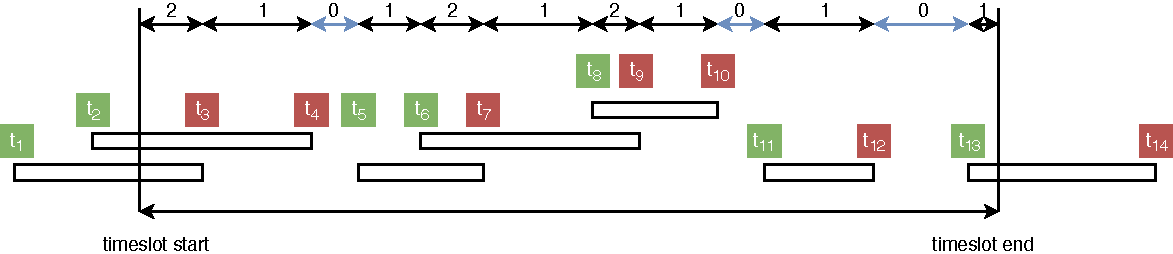
\includegraphics[width=\textwidth]{figures/utilization_rate}
    \caption{Utilization rate during a time period where the top numbers indicate the workload for sub-periods of time}
    \label{fig:utilization_rate}
\end{figure}

\todo{add visualizations of utilization}

\section{Work-allocation patterns}
Finally, all this information can be used to mine resource allocation patterns. The exact input data depends on which resource-allocation patterns should be mined. 

\todo{Implement and report}






\clearemptydoublepage

% \chapter{Visualization definition}\label{chapter:visdef}
% This chapter contains a brief overview inclusive description and definition of various inter-case resource dependency visualizations. First of all, in this context resources are described as durable resources, i.e resources that are assigned and released from events, but are neither destroyed or created.

\section{Resource Workload}
This section discusses several resource workload related visualizations. Resource workload is defined as the amount of events a resource is working at simultaneously for a certain point of time. This is a continuous value over time for each resource. Equation \ref{def:workload} defines the workload for a certain resource $r$ for time $t$, where $t \in l_T$. $l_T = \{\#_t(e) | e \in l \}$ being the set of all timestamps in event log $l$ and $E \in l$ being all events in event log L ordered ascending by $\#_{ts}(e)$ , i.e. chronologically by start date. The notation used in this thesis for selecting an event, case and log attributes it the following: $\#_{attribute}(object) = value$ and defined by \cite{aalst2016process}.

The sets $se$ and $ce$ are defined as a set of activity life-cycle transitions which denote the start and completion of an activity life-cycle, respectively. $\#_{ts}(e)$ denotes the time of the first occurrence of a start activity life-cycle transition for event instance $e$. Similarly, $\#_{te}(e)$ denotes the time of the last occurrence of a completion activity life-cycle transition for event instance $e$. Furthermore, $\#_{ts}(c)$ and $\#_{te}(c)$ denote the case start and end times, i.e. the time when the first event of the case was started, and the time when the last event of the case ended. The same applies for $\#_{ts}(l)$ and $\#_{te}(l)$ for the event log $l$. Note that the time dimension is simplified to be a discrete variable starting from $0$ for the first timestamp which is similar to \cite{aalst2016process}. The exact timestamp is not of importance in this context, only the relative time difference which can be illustrated in the simplified discrete setting.  

\begin{equation}\label{def:workload}
  \begin{array}{l}
    workload(r,t) =  
    | \{e \in l | \; \#_{ts}(e)  \leq t \leq \#_{te}(e) \wedge \#_r(e)=r\}| \; 
  \end{array}
\end{equation}

% \begin{figure}[h]
% 	\centering
%     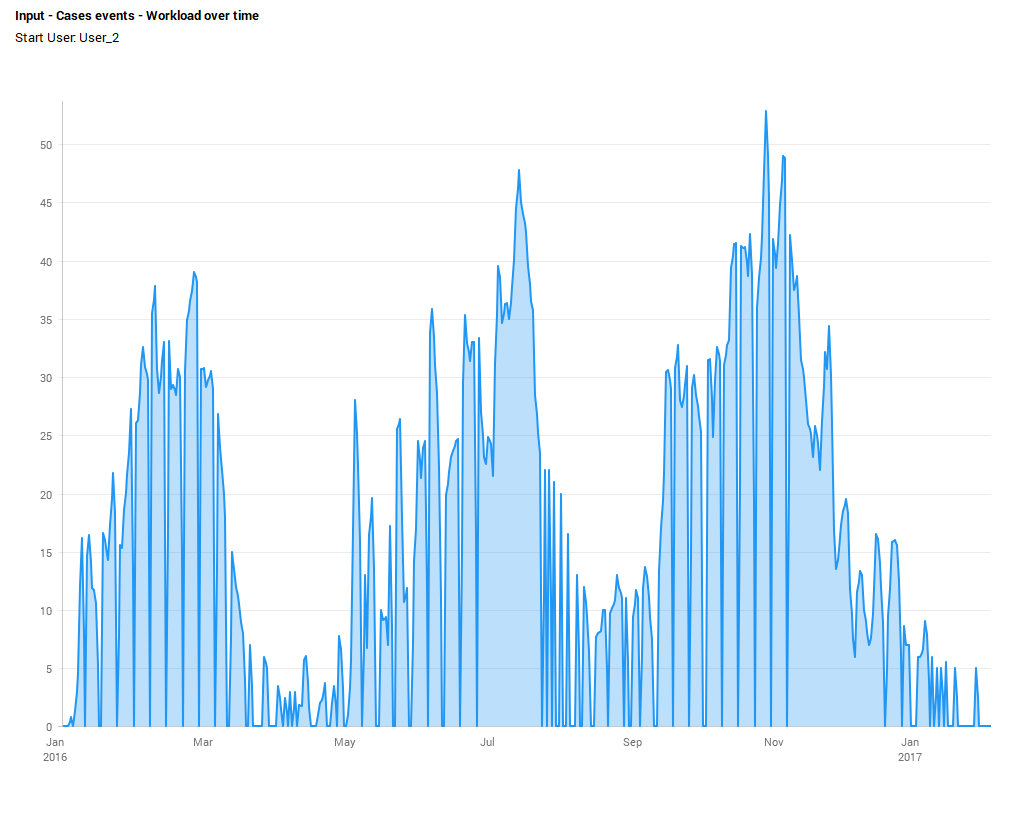
\includegraphics[width=.8\textwidth]{figures/workload.png}
%     \caption{Workload over time for User\_2 of the BPI Challenge 2017 event log.}
%     \label{fig:workload}
% \end{figure}

\begin{figure}[h]
	\centering
    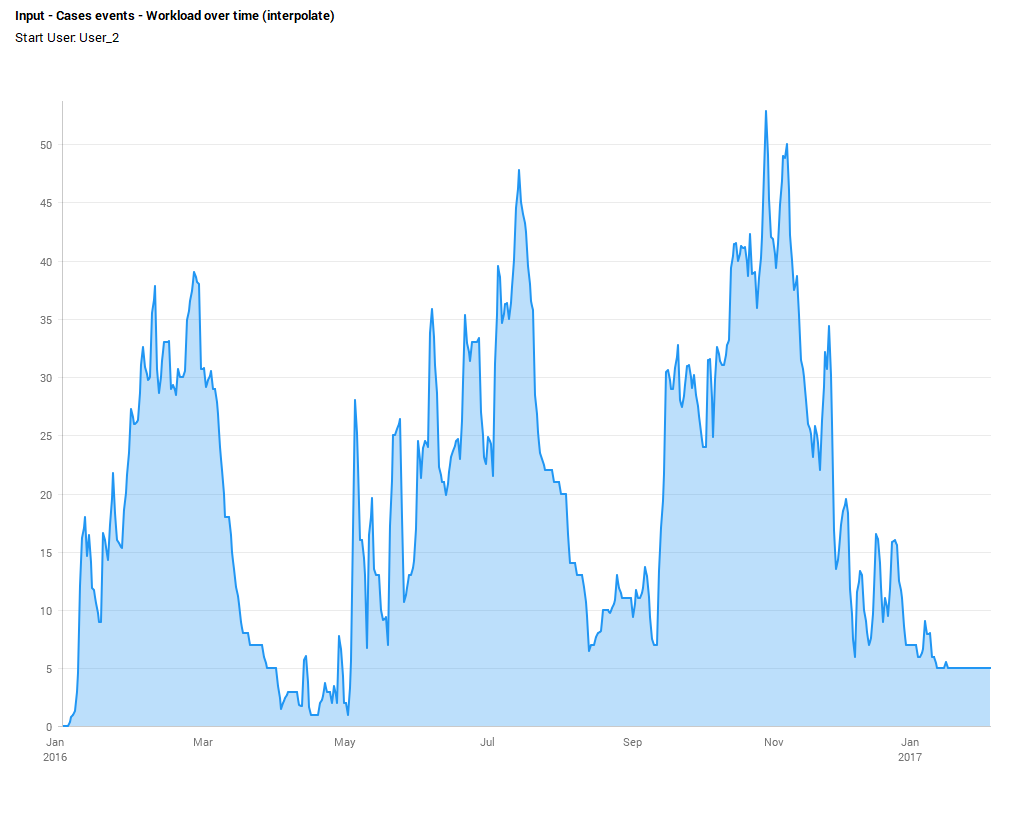
\includegraphics[width=\textwidth]{figures/workload_interpolate.png}
    \caption{Workload over time for User\_2 of the BPI Challenge 2017 event log.}
    \label{fig:workload}
\end{figure}

Figure \ref{fig:workload} illustrates the workload over time of the resource User\_2 for the complete period of the event log. The workload varies from fifty-three events to zero events. 

% The figure also shows a lot of downwards spikes to zero. This is because equation \ref{def:workload} returns zero when no events are performed by a resource for a specific period (in the case of Figure \ref{fig:workload}, the workload is calculated per day). However, this is incorrect, because the workload does not decrease to zero when no events are performed. Instead, the workload remains equal when no events are performed, i.e. the last non-zero workload value should be used. This is shown for the same data in Figure \ref{fig:workload_interpolate}. Equation \ref{def:amount} counts the number of events for a resource in a certain period and Equation \ref{def:workloads} simply returns all periods of minimal size of an event log.

% \begin{equation}\label{def:amount}
%     count(r,t_s,t_e) =  | \{e \in E | t_s \leq e_t \leq t_e \wedge e_r=r\}|
% \end{equation}

% \begin{equation}\label{def:workloads}
%     workloads(r) =  \{workload(r,t_s,t_s+1) | t_s \in t\}
% \end{equation}

% \begin{equation}\label{def:workload_interpolated}
%   \begin{array}{l}
%     workload\_in(r,t_s,t_e) =  
%     \begin{cases}
%     	workload(r,t_s,t_e) & \quad \text{if }  count(r,t_s,t_e) > 0 \\
%         workloads(r)_n \; s.t. \; \forall m \in t, m \leq n \wedge workloads(r)_m \leq t_s & \quad \text{if }  count(r,t_s,t_e) = 0
%     \end{cases}
%   \end{array}
% \end{equation}

\subsection{Resource Workload per Case}
In order to correlate the resource workload with case-specific variables, such as case outcome, it is necessary to calculate the average workload of users during a case execution. Equation \ref{def:workload_case} calculates the average workload of a single resource during a case execution by simply calculating all workloads and dividing by the number of workloads. Note that the workload is calculated for all points in time during the case execution. 

\begin{equation}\label{def:workload_case}
    avg\_wl\_during\_case\_resource(c, r) = \cfrac{\sum_{t=\#_{ts}(c)}^{\#_{te}(c)} workload(r,t)}{\#_{te}(c)-\#_{ts}(c)}
\end{equation}

Finally, Equation \ref{def:workload_case_resources} averages all the workloads for each resource working on the case, thus resulting in the overall average of the average workload for all resources during case execution. This overall average can give an indication of how busy the resources are during the case and might be used to correlate it with other variables such as case outcome. The latter is described in the next section. Note that $res(c)$ is defined as $res(c) = \{\#_{r}(e) | e \in c\}$ and $res(l) = \bigcup_{c \in l} res(c)$ for case $c$ and event log $l$, respectively. The methods simply return all resources which are associated with a case or log. 

\begin{equation}\label{def:workload_case_resources}
     avg\_workload\_case(c) = \cfrac{\sum_{r \in res(r)} avg\_workload\_case\_resource(c, r) }{|res(c)|}
\end{equation}

\subsection{Correlating Variables to Resource Workload}
This section elaborates on the previous sections by correlating the average case workload of all resources against other variables. An interesting correlation might be to correlate the average workload against the case outcome. For the BPIC 2017 dataset, which is about loan requests, the case outcome is either: \textit{success} when the loan request is accepted, \textit{denied} when the loan request is denied, \textit{cancel} when the loan request is either cancelled or the customer/bank did not reply in time or \textit{error} when no other outcome applies. The latter can occur because the case is not correctly closed due to administrative issues, or the case is not yet finished.

\begin{figure}[h]
	\centering
    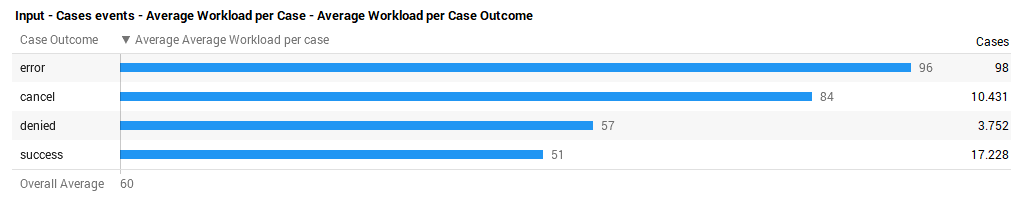
\includegraphics[width=\textwidth]{figures/workload_case_outcome.png}
    \caption{Average workload for each case outcome}
    \label{fig:workload_case_outcome}
\end{figure}

Figure \ref{fig:workload_case_outcome} shows the average workload with respect to case outcome. The average workload is calculated by simply averaging all case workloads with a certain outcome as is defined in Equation \ref{def:workload_case_outcome}. Figure \ref{fig:workload_case_outcome} shows a correlation between low average workload and successful loan request outcomes. Higher average workloads are correlated with denied and cancel outcomes (and error, but the amount of cases is relatively low). This could imply that when resources are very busy, i.e. have a high workload, the probability is higher than a case is cancelled. This might be the case because e.g. the resources do not have time to respond quickly so the customer in time so the customer finds another bank for their loan request.  

\begin{equation}\label{def:workload_case_outcome}
     avg\_workload\_case\_outcome(outcome) = \cfrac{\sum_{\{c \in l | \#_{outcome}(c)=outcome\}} avg\_workload\_case(c) }{|\{c \in l | \#_{outcome}(c)=outcome\}|}
\end{equation}

\begin{figure}[h]
	\centering
    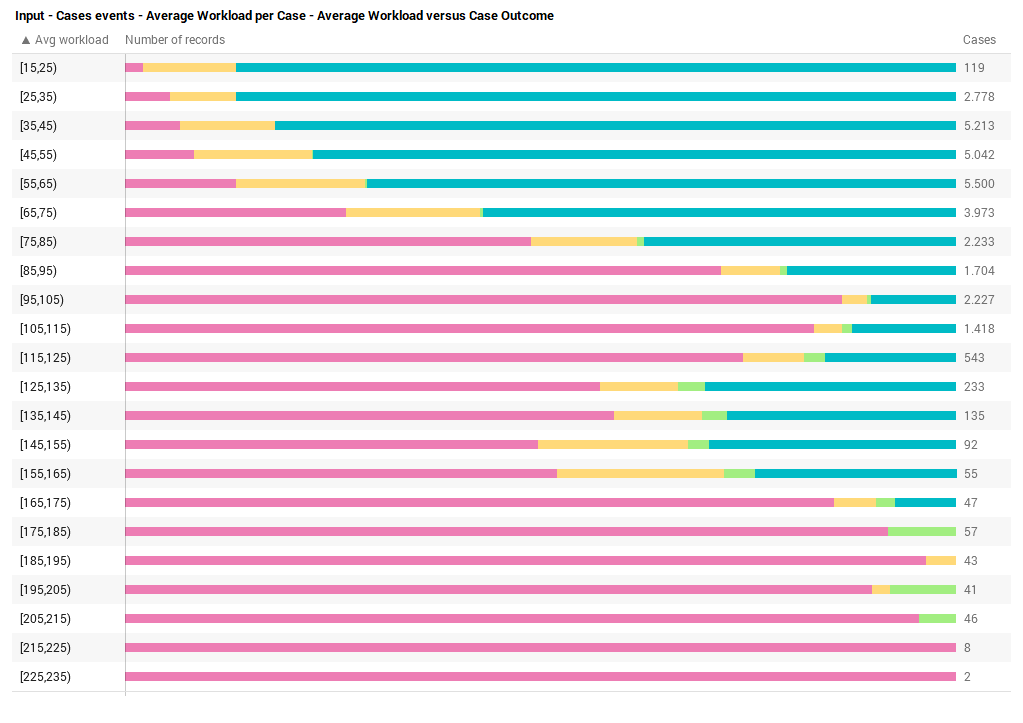
\includegraphics[width=\textwidth]{figures/workload_groups_case_outcome.png}
    \caption{Average workload with respect to case outcome}
    \label{fig:workload_groups_case_outcome}
\end{figure}

Figure \ref{fig:workload_groups_case_outcome} elaborates on Figure \ref{fig:workload_case_outcome} by splitting the cases into groups of average workload and showing the relative amount of case outcomes. The case outcome is shown in colours, whereas red represents \textit{cancel}, yellow represents \textit{denied}, green represents \textit{success} and light-green represents \textit{error}. The Figure shows that there is a clear connection between higher workload and higher relative size of \textit{cancel} outcomes.

It is very interesting that this trend does not completely hold because of the workload 125 until 165. This might however be an instance of the Yerkes–-Dodson law of arousal which indicates that there is a bell-shaped curved relation between workload and performance. More research is required in order to validate this.  

\subsection{Comparing workload between resources}

\subsection{Comparing workload between cases}

\section{Performance}
This section describes the performance metric for resources. the first section describes definitions which are used in the visualizations of the second section. 

\subsection{Definition}
The performance metric is defined for a certain resource for a certain point in time $t$. The performance measure simply counts the number of events which an employee completes on a point in time and is defined in Equation \ref{def:performance}. Note that trivially $\#_{ts}(l) \leq t \leq \#_{te}(l)$ should be the case.

\begin{equation}\label{def:performance}
  \begin{array}{l}
    performance\_completed(r,t) = 
   | \{e \in l | \#_{te}(e) = t \wedge \#_{r}(e)=r \}| 
  \end{array}
\end{equation}

Because time is a continuous value, it might not make sense to limit the performance to only a single point in time. Therefore, Equation \ref{def:performance_period} defines the performance for a certain resource on a specific period where $t_s$ is the start of the period and $t_e$ is the end of the period. The Equation is simply a sum over the time period for Equation \ref{def:performance}. Note that it should be the case that $\#_{ts}(l) \leq t_s \leq t_e \leq \#_{te}(l)$.

\begin{equation}\label{def:performance_period}
  \begin{array}{l}
    performance\_completed\_period(r,t_s, t_e) = \sum_{t = t_s}^{t_e} performance(r,t)
  \end{array}
\end{equation}

Equation \ref{def:events_started} describes the opposite of Equation \ref{def:performance}, namely the number of events which are started and allocated to a specific resource $r$ on a certain period in time $t$. The length of the worklist in Equation \ref{def:worklist} is calculated, because the worklist contains all 'open', i.e. unfinished tasks, for a certain resource. Equation \ref{def:events_started_period} is similar to Equation \ref{def:performance_period} and again is simply the sum over a period of time which generates the number of started events for a period.

\begin{equation}\label{def:events_started}
  \begin{array}{l}
    performance\_started(r,t) =
   | \{e \in l | \#_{ts}(e) = t \wedge \#_{r}(e)=r \}| 
  \end{array}
\end{equation}

\begin{equation}\label{def:events_started_period}
  \begin{array}{l}
    performance\_started\_period(r,t_s,t_e) = \sum_{t = t_s}^{t_e} events\_started(r,t)
  \end{array}
\end{equation}

Finally, Equation \ref{def:workload_delta} describes the change in workload for a certain resource on a point in time. When the workload delta yields a positive value, the workload of a resource increases, whereas negative values imply that the workload of a resource decreases. Equation \ref{def:workload_delta} is a simply the difference between Equation \ref{def:events_started} and Equation \ref{def:performance}. Equation \ref{def:workload_delta_period} is again the sum over a period of Equation \ref{def:workload_delta}.

\begin{equation}\label{def:workload_delta}
  \begin{array}{l}
    workload\_delta(r,t) =  performance\_started(r,t) - performance\_completed(r,t) 
  \end{array}
\end{equation}

\begin{equation}\label{def:workload_delta_period}
  \begin{array}{l}
    workload\_delta\_period(r,t_s,t_e) = \sum_{t = t_s}^{t_e} workload\_delta(r,t)
  \end{array}
\end{equation}


\subsection{Visualization}
This section elaborates on the definitions of the previous section by using them in several visualizations. This section presents rather simple, yet useful visualizations for resource performance. 

Figure \ref{fig:tasks_started} illustrates the tasks started summed for all resources. The graph distinguishes automated and manual events. Automated events are defined as events which take less than thirty seconds or contain only an end activity life-cycle activity. The Figure shows that the automated events closely follow the manual events, i.e. for each manual event, multiple automated events are performed. Further investigation validates that this is indeed the case.   

The Figure shows a clear pattern which is distinctive for the BPI Challenge 2017 dataset. It appears that almost no events arrive during the weekends (which is not uncommon for banks due to their limited opening hours) and that the events stream starts on Monday. Figure \ref{fig:dayofweek} supports this assumption by showing the average difference between started events of a day compared to the previous day. The Figure clearly shows that on Monday, much more events are started than the day before. Tuesday until Friday are rather stable, meaning that not almost the same amount of events are started as on Monday. Thursday seems to have a small decrease in events compared to Wednesday. This means that the amount of events peak, on average, each Wednesday. As expected, in the Weekend, significant fewer events are started than during the week. 

\begin{figure}[h]
	\centering
    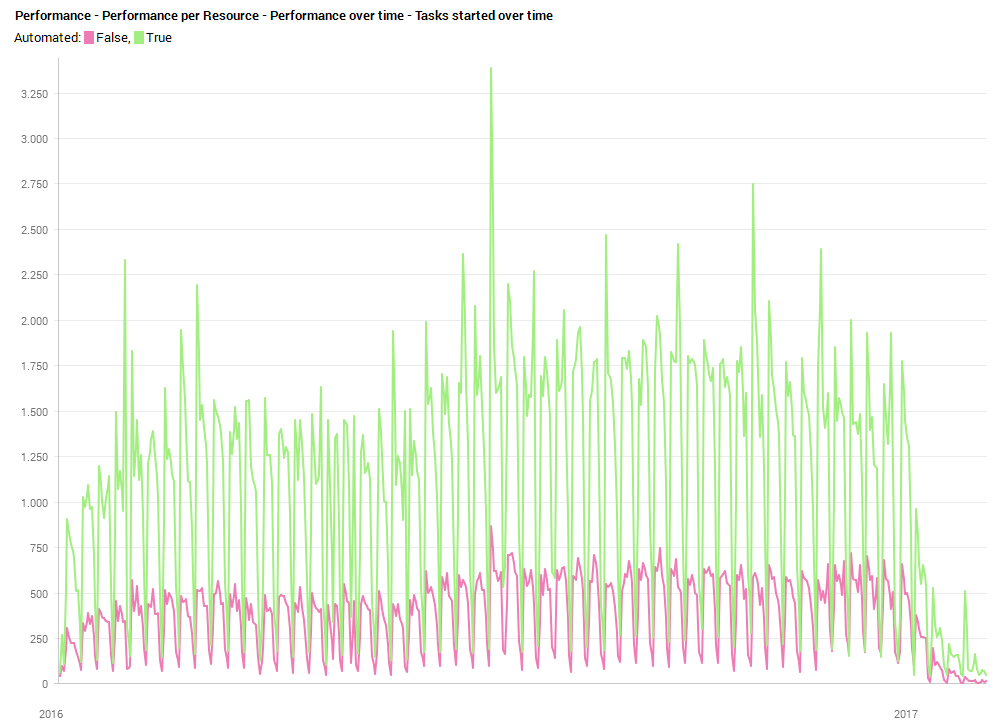
\includegraphics[width=0.9\textwidth]{figures/tasks_started.png}
    \caption{Tasks started over time for the BPIC2017 log.}
    \label{fig:tasks_started}
\end{figure}

\begin{figure}[h]
	\centering
    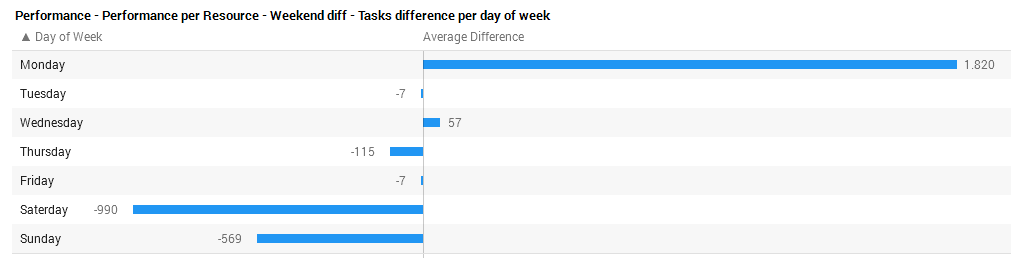
\includegraphics[width=0.9\textwidth]{figures/dayofweek.png}
    \caption{Average tasks started difference per weekday with respect to the previous weekday.}
    \label{fig:dayofweek}
\end{figure}

Figure \ref{fig:performance} shows a similar pattern as Figure \ref{fig:tasks_started} and describes the amount of events completed for each day. The Figures appear to closely follow each other, i.e. when more tasks are started, more tasks are completed. This could indicate that there is a sufficiently large pool of resources available which can handle all incoming cases. 

\begin{figure}[h]
	\centering
    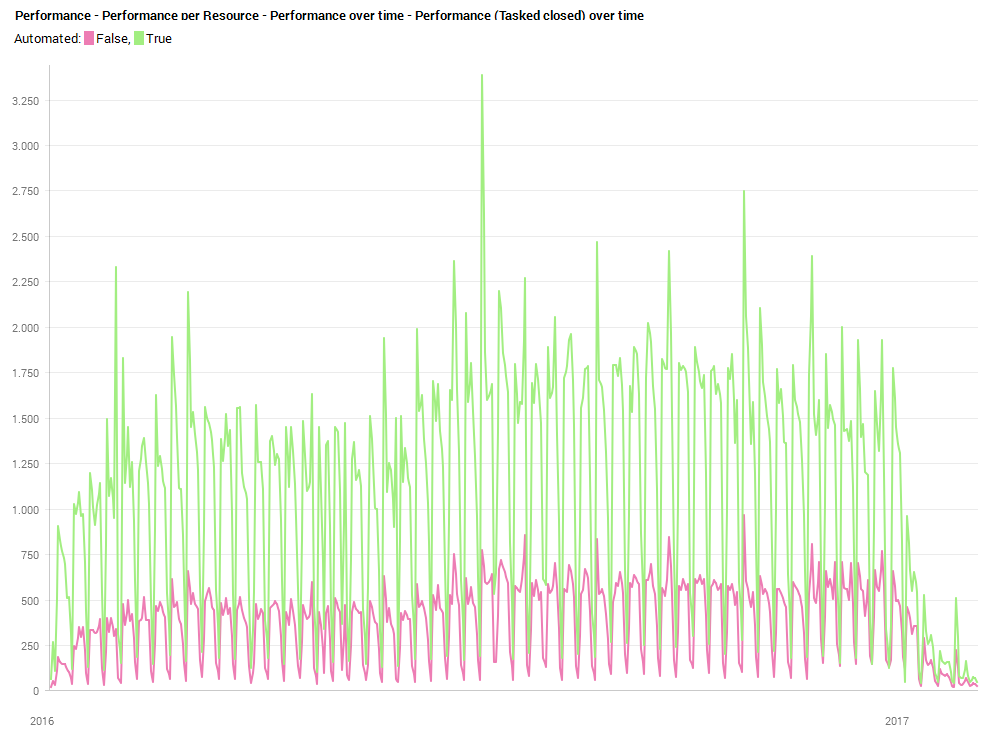
\includegraphics[width=0.9\textwidth]{figures/performance.png}
    \caption{Tasks completed (performance) over time for the BPIC2017 log.}
    \label{fig:performance}
\end{figure}

Figure \ref{fig:workload_delta} illustrates the difference between the tasks started and the tasks completed for all days. It shows that in general, the workload is rather stable, i.e. not many tasks are left open for a long time because after each positive spike, a negative spike occurs. This can be seen especially in the middle of the graph, where after a long period of positive workload delta values, a large negative correction occurs. Note that this is during the holiday period (June, July) and that the process might be handled differently than normally. 

At the beginning and end of the dataset, a large period of positive and negative workload delta appears. This is probably is because of the case filtering, namely: at January 2016, employees might be working on finishing cases of 2015 which are filtered from the log. The same appears at the end of the log, namely that employees might be already working on cases which arrive in 2017 but are also not part of the log. Finally, an interesting pattern is that at approximately the 21$^{st}$ of each month a large negative correction takes place. This might imply that during this date many events are completed using batch processing. 

\begin{figure}[h]
	\centering
    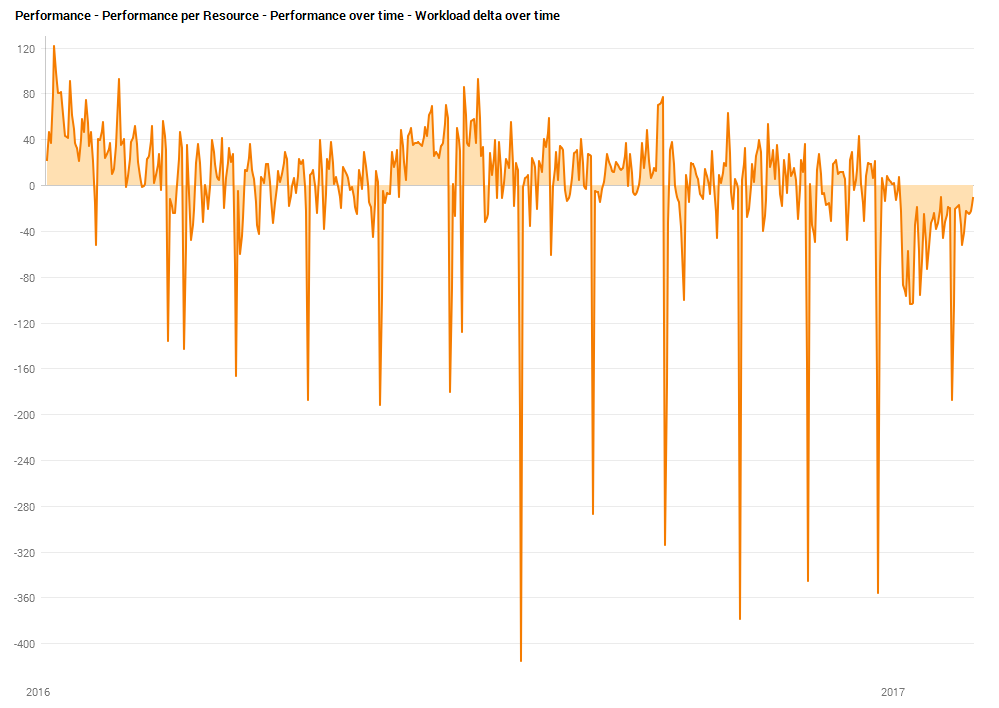
\includegraphics[width=0.9\textwidth]{figures/workload_delta.png}
    \caption{Workload delta over time for the BPIC2017 log.}
    \label{fig:workload_delta}
\end{figure}

\section{Resource Prioritization Policies}
This section discusses several prioritization policies visualizations. Prioritization Policies are general methods which resources can follow in order to define what their next task is. Resources each have a WorkList, which is an ordered queue of tasks which are allocated to a resource. WorkList $wl$ is ordered on arrival of tasks and contains all open (i.e. unfinished) tasks of a single resource. $\#_{wl}(r)$ denotes the WorkList of resource $r$. 

Each resource might use a different prioritization policy, or this policy might be fixed for certain groups of resources/departments. Either way, it might be interesting to analyse the which resource prioritization policy is used, and what effect it has on the process. The next section describes the definitions necessary for the visualization of the resource prioritization policies. The next section shows and describes the visualizations. 

\subsection{Definitions}

The first step is to calculate the WorkList at all points in time for each resource. This is important because the WorkList is the basis for calculating which resource prioritization policy is used. The $worklist(r, t)$ function requires a resource and a point in time, whereas $\#_{ts}(l) \leq t \leq \#_{te}(l)$. Equation \ref{def:worklist} describes this function. The function simply lists all events where $\#_{ts}(e) \leq t$, i.e. the events start before or on time $t$ where $t < \#_{te}(e)$, i.e. the events end after time $t$. In other words, it lists all open tasks at point $t$. This function is abbreviated to $wl(r,t)$.

\begin{equation}\label{def:worklist}
  \begin{array}{l}
    worklist(r, t) =  \{e \in l |\; \#_r(e) = r \wedge \#_{ts}(e) \leq t < \#_{te}(e)   \}
  \end{array}
\end{equation}

% Old recursive function
% \begin{equation}\label{def:worklist}
%   \begin{array}{l}
%     worklist(r, t) =  
    
%     \begin{cases}
%     worklist(r, t -1) + \{e \in E | e_r = r \wedge e_l \in se & \text{for } t \leq t_s \\ 
%      \wedge   e_t = t \} - \{e \in E | e_r = r 
%     \wedge e_l \in ee \wedge e_t = t\} \\ 
%     [ \; ], & \text{for } t < L_ts
%   \end{cases}
%   \end{array}
% \end{equation}

A method to see how much a certain resource follows a prioritization policy is to define a penalty function for all policies. The policy with the lowest penalty is then followed best. Equation \ref{def:fifo} defines the penalty function of FiFo and checks whether there exist events at all for time $t$, otherwise, the penalty is simply zero. Furthermore, it is checked whether the worklist has at least more than one item, otherwise, the penalty is also zero. The latter is the case that the penalty does not make sense when the worklist contains zero or one items because one cannot prioritize a single item. 

If there exist any events, the $fifo\_penalty(r,e)$ function is called for each event the results are summed up. Note that $wlr$ is defined as $wlr = wl(r, \#_{te}(e))$ The $fifo\_penalty(r,e)$ in Equation \ref{def:fifo_penalty} first checks whether the event exists in the workload (which should always be the case for non-automated events, otherwise an event has not been started, only completed), if not zero is returned. In all other cases, the FiFo penalty is defined as the size of the worklist minus the index of the event defined by the worklist size. The latter step is to normalize the error, otherwise, a high worklist might imply higher violations. The Equation shows a linear normalization, but other normalizations can also be considered. When the index is high, i.e. the event has just been added to the worklist, the penalty is lowest, while when the index is low, i.e. when many more events have been added after the event start, the penalty is high.     

\begin{equation}\label{def:fifo}
  \begin{array}{l}
    fifo\_error(r, t) = 
    
    \begin{cases}
    	0, & \text{for } \exists{e \in l} | \; \#_{te}(e) = t \wedge \#_r(e)=r \\
        \sum_{\{e \in l | \#_{r}(e)=r \wedge \#_{te}(e)=t \}} fifo\_penalty(r,e)  & \text{otherwise}
    \end{cases}
  \end{array}
\end{equation}


\begin{equation}\label{def:fifo_penalty}
  \begin{array}{l}
    fifo\_penalty(r, e) = 
    \begin{cases}
    	0, & \text{for } |wlr| \leq 1 \wedge e \in wlr  \\
        \cfrac{|wlr| - |\{w \in wlr\; \#_{ts}(w)  \leq \#_{ts}(e)\}|}{|wlr|}  & \text{for } |wlr| > 1 \wedge e \in wlr
    \end{cases}
  \end{array}
\end{equation}

The same can be done for the LiFo penalty, only slightly simpler. Equation \ref{def:lifo} is almost equal to \ref{def:fifo}, instead, Equation \ref{def:lifo_penalty} is called instead of Equation \ref{def:fifo_penalty}. The only difference between the latter two equations is that the penalty is calculated by simply finding the index of the event in the worklist of the corresponding resource. This has the opposite effect as the fifo penalty, such that the penalty is high when the index is high, i.e. the event has just been added, and is low when the index is low, i.e. many events are added after the event has been started. This is exactly the difference between FiFo and LiFo. 

\begin{equation}\label{def:lifo}
  \begin{array}{l}
    lifo\_error(r, t) = 
    
    \begin{cases}
    	0, & \text{for } \exists{e \in l} | \; \#_{te}(e) = t \wedge \#_{r}(e)=r \\
        \sum_{\{e \in l | \#_{r}(e)=r \wedge \#_{te}(e)=t\}} lifo\_penalty(r,e)  & \text{otherwise}
    \end{cases}
  \end{array}
\end{equation}


\begin{equation}\label{def:lifo_penalty}
  \begin{array}{l}
    lifo\_penalty(r, e) = 
    
    \begin{cases}
    	0, & \text{for } |wlr| \leq 1 \wedge e \in wlr  \\
        \cfrac{|\{w \in wlr|\; \#_{te}(w)  \leq \#_{ts}(e)\}|}{|wlr|}  & \text{for } |wlr| > 1 \wedge e \in wlr
    \end{cases}
  \end{array}
\end{equation}

Finally, the last prioritization policy is Shortest Task in Queue and requires a slightly different penalty function. Note that $\#_{td}(e)$ is defined as $\#_{td}(e)=\#_{te}(e)-\#_{ts}(e)$, i.e. the duration of event $e$. Equation \ref{def:shortenalty} requires the construction of an ordered list of event durations, whereas each event in the worklist has exactly one corresponding duration value (i.e. end time minus start time). This means that the lowest durations have the lowest index and thus also the lowest penalty. 

\begin{equation}\label{def:short}
  \begin{array}{l}
    short\_error(r, t) = 
    
    \begin{cases}
    	0, & \text{for } \exists{e \in l} | \; \#_{te}(e) = t \wedge \#_{r}(e)=r \\
        \sum_{\{e \in l | \#_{r}(e)=r \wedge \#_{te}(e)=t\}} short\_penalty(r,e)  & \text{otherwise}
    \end{cases}
  \end{array}
\end{equation}

\begin{equation}\label{def:shortenalty}
  \begin{array}{l}
    short\_penalty(r, e) = 
    
    \begin{cases}
    	0, & \text{for } |wlr| \leq 1 \wedge e \in wlr  \\
        
        \cfrac{|\{w \in wlr|\; \#_{td}(w) \leq \#_{td}(e)\}|}{|wlr|}  & \text{for } |wlr|> 1 \wedge e \in wlr\\
    \end{cases}
  \end{array}
\end{equation}

\subsection{Visualization}
This section elaborates on the definitions of the last section by showing several visualizations based on the definitions. Figure \ref{fig:error_total} shows the total error for the FiFo, LiFo and Shortest Job First scheduling policies for the BPIC 2017 dataset. The weekly spikes are a noticeable artefact for this dataset. It appears that resources acquire their workload on Monday of all cases which arrived during the weekend and work their way through the worklist during the week. At the end of the week, the worklists are almost empty and no tasks are performed during the weekend. This pattern can also clearly be seen in Figure \ref{fig:error_total}.

\begin{figure}[h]
	\centering
    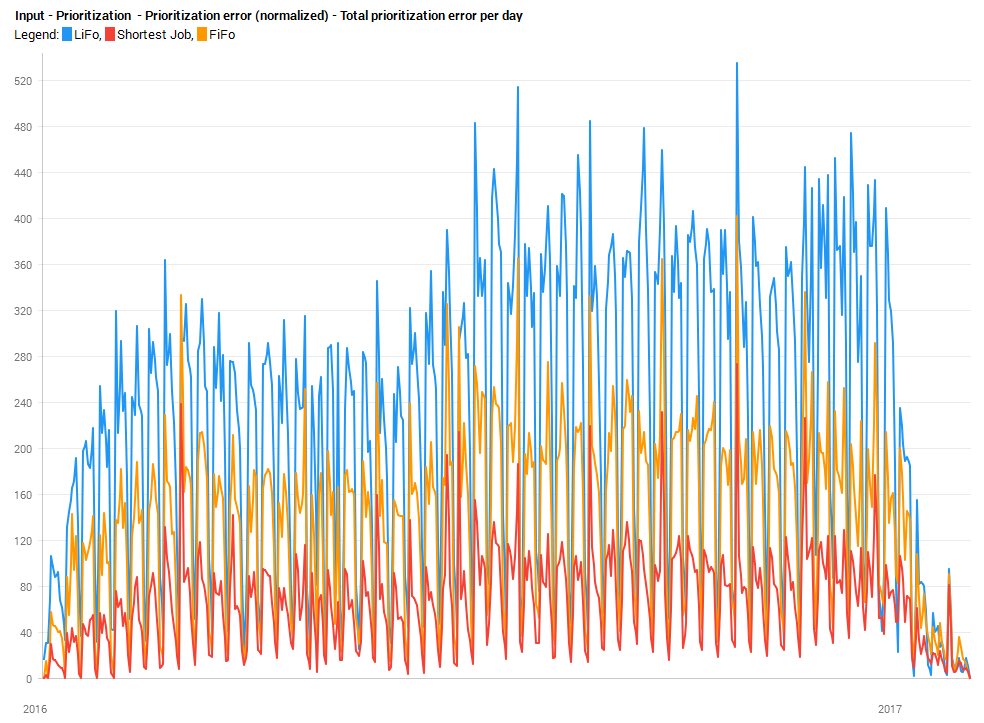
\includegraphics[width=0.9\textwidth]{figures/total_prioritization_error.png}
    \caption{Total FiFo, LiFo and shortest job error of BPIC2017 per day.}
    \label{fig:error_total}
\end{figure}

When inspecting the figure briefly, it can be seen that, on average, the LiFo penalty seems to be highest at most times, while the Shortest Job First error seems lowest at almost all times. The FiFo error is in between these two errors. This indicates that the prioritization is executed more accordingly to the Scheduled Job First policy, than according to the LiFo policy. Furthermore, one can notice no significant changes over time, expect at the begin and end of the log where there are sudden decreases and increases. This is however the effect of a case filter which removes all open cases in the event log. 

The average FiFo penalty is 0.044, and in 112,293 event instances, a FiFo penalty was given. Thus indicating that in these event instances FiFo was not fully followed. For LiFo, the average error is 0.074 and the amount of event instances with a penalty is 141,949. Compared to FiFo, LiFo has both a higher average error and more event instances which have a LiFo error. Thus indicating that the prioritization schedule is more likely to follow FiFo than LiFo. Finally, the average Shortest Job First penalty is 0.021507 and the amount of event instances which have a penalty is 89,650. Both values are significantly lower compared to LiFo and FiFo, thus indicating that this scheduling method might be a better fit. 


\begin{figure}[h]
	\centering
    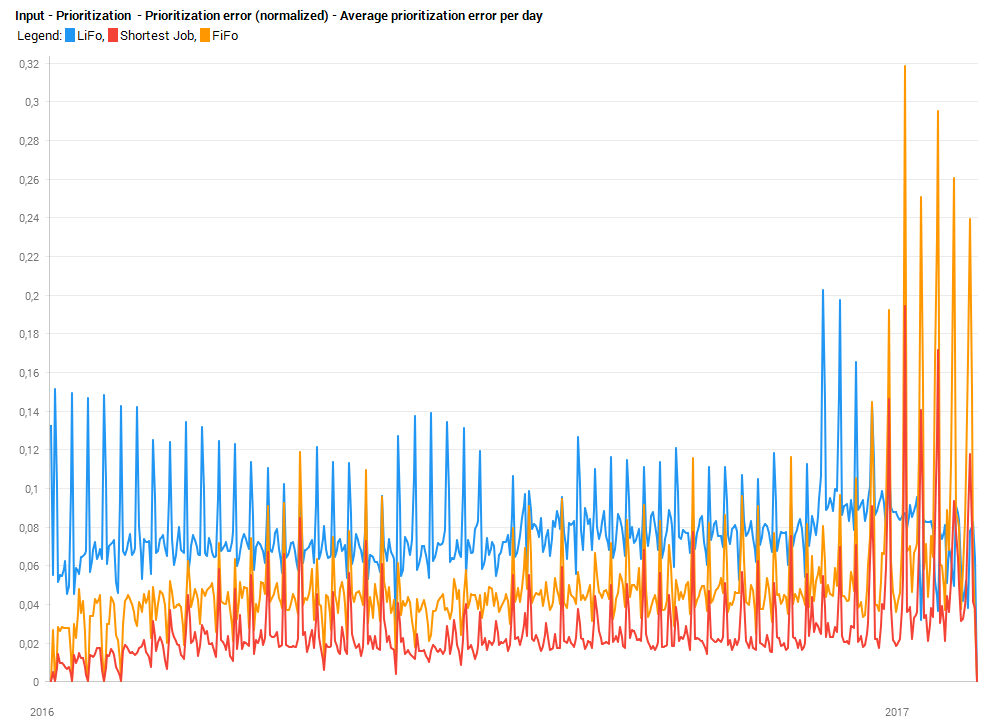
\includegraphics[width=0.9\textwidth]{figures/avg_prioritization_error.png}
    \caption{Average FiFo, LiFo and shortest job penalty of all events for BPIC2017 per day.}
    \label{fig:error_avg}
\end{figure}

Another way of visualizing the prioritization penalties is by taking the average penalty per event and is shown in Figure \ref{fig:error_avg}. This Figure contains the same finding as \ref{fig:error_total} that most of the time, the Shortest Job First policy seems to be followed best and the LiFo policy seems to be followed least. However, this Figure contains an interesting increasing trend at the end of the dataset, where the average LiFo error decreases and the Shortest Job First and FiFo policies significantly increase.  

Finally, Figure \ref{fig:error_avg_nnull} is similar to Figure \ref{fig:error_avg}, expect from the fact that only the non-zero penalties are taken into account. In other words: the Figure contains the average of all events which do not strictly follow the prioritization policy. This shows that, except the last months, the LiFo is close to the maximum of one, meaning that the LiFo scheduling policy is not followed at all. 

\begin{figure}[h]
	\centering
    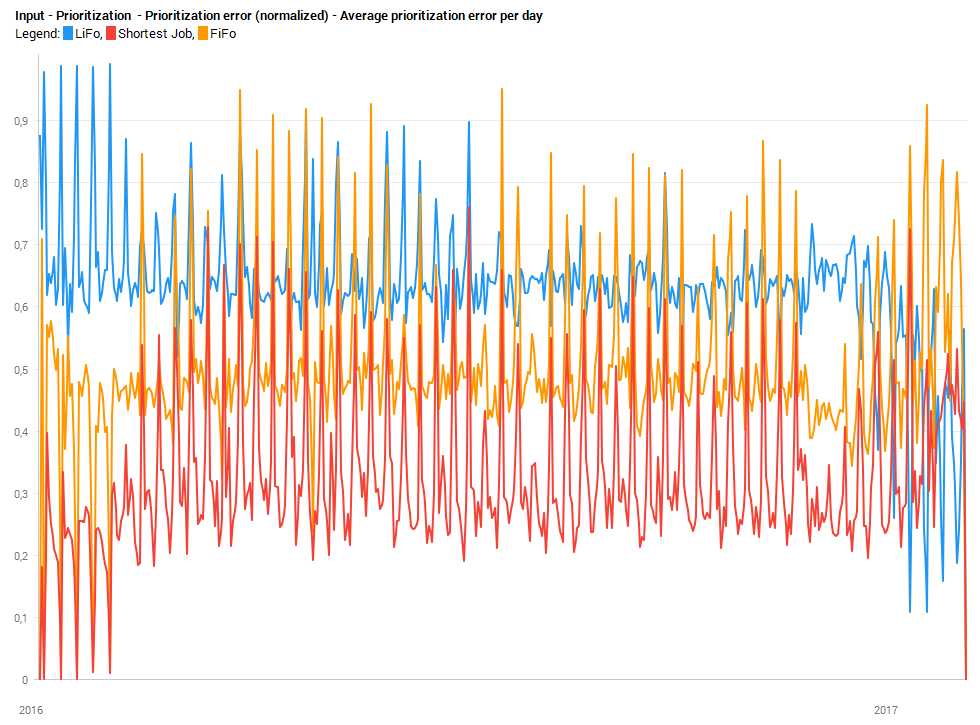
\includegraphics[width=0.9\textwidth]{figures/avg_error_nnull.png}
    \caption{Average FiFo, LiFo and shortest job penalty of all non-zero penalties for BPIC2017 per day.}
    \label{fig:error_avg_nnull}
\end{figure}

\section{Annotating Process Models}

\chapter{Implementation}\label{chapter:implementation}

\begin{itemize}
    \item 
\end{itemize}

\clearemptydoublepage

\chapter{Evaluation}\label{chapter:evaluation}
\input{chapters/evaluation}

\clearemptydoublepage

% \chapter*{Inter-case resource pattern}\label{chapter:case_studies}
% \section*{Case Studies}

This main subject of this thesis is inter-case resource patterns and consists of the following parts: role mining, resource bottleneck and work-allocation patterns analysis. Role Mining aims to identify the roles of resources based on their behaviour. Resource Bottleneck analysis looks at the availability and workload of resources and aims to find bottlenecks in a process by analysing resources and roles. Finally, work-allocation patterns aims to check if resources and roles follow certain patterns, such as for example: handling tasks in a First-in-First-out (FiFo) or Last-in-First-out (LiFo) manner. The analysis, furthermore, looks at why resources sometimes deviate from their common behaviour. The following sections describe how a case study can be approached for the subjects in this thesis. 

% There are two main reasons for conducting case studies, namely: to ensure that the analysis can be use in practise and to validate the results of the analysis techniques. 



\subsection*{Role Mining}
Role Mining only requires an event log where each event is related to a resource.  The case study starts with a demo of the proof-of-concept for the client including an interview to gather domain knowledge. Next, a role mining analysis is conducted by the student or by the customer and the results are shared with a domain expert. The domain expert can validate the findings of the role mining analysis by comparing the results with its organizational structure and domain knowledge. If the student is not authorized to use the client data, the role mining analysis framework is explained to the client and the client can perform the analysis theirself. 


% There are two possible methods to perform  role mining in a case study depending on whether the student and consultant are authorized to use the client data. In both cases, the case study starts with a demo of the proof-of-concept for the client including an interview to gather some domain knowledge about the process. 

% If the student/consultant is authorized to use the client data, a role mining analysis can be conducted by the student/consultant and the results are shared with a domain expert. The domain expert can validate the findings of the role mining analysis by comparing the results with its organizational structure and domain knowledge. This process might be iterative, in other words: the analysis could be adapted based on feedback of the domain expert to optimize the analysis. 

% If the student is not authorized to use the client data, the role mining analysis framework is explained to the client after the demo. The proof-of-concept is than deployed such that it is able to use the client's data. The client can then perform the role mining analysis themself including a validation of the results (e.g. comparing the results against their security policy). Afterwards, the client is interviewed again and the findings of the role mining are shared.

\subsection*{Resource Bottleneck Analysis}
% The resource bottleneck analysis case study is slightly different from the role mining case study because it consists of a set of dashboards instead of an algorithm. 

The bottleneck analysis requires an event log containing events which are related to resources and preferably event start and event end times. The case study starts with a demo of the proof-of-concept including an interview to gather domain knowledge. The client, furthermore, gets a training/workshop on how to use the dashboards and the proof-of-concept is deployed such that it is able to use the client's data. The client can then perform the resource bottleneck analysis on its own data and the findings are afterwards evaluated. 

% The findings include the usefulness of the analysis, the correctness of the analysis and the user experience. 

% Furthermore, it is optional that the resource roles are known and the resource availability is known. 



% If the student/consultant are authorized to use the client data, they can walkthrough the bottleneck analysis together with the client. 


\subsection*{Work-allocation patterns}
The work-allocation pattern case study is similar to the resource bottleneck analysis case study. However, this analysis can be tailored to the client's requirements by analysing patterns which are specific to the client. The standard work-allocation patterns include whether resources follow FiFo, LiFo, Shortest-Job-First, Closest-Deadline-First prioritization patterns. However, the client can define their own patterns which can be implemented specifically for the customer.  The data required for this case study depends on the client's work-allocation patterns. The standard patterns require an event log which contains a related resource per event including event start and event end times. 

\chapter*{Inter-case resource patterns}
This main subject of this thesis is inter-case resource patterns and consists of the following parts: role mining, resource bottleneck and work-allocation patterns analysis. Role Mining aims to identify the roles of resources based on their behaviour. Resource Bottleneck analysis looks at the availability and workload of resources and aims to find bottlenecks in a process by analysing resources and roles. Finally, work-allocation patterns analysis aims to check if resources and roles follow certain patterns, such as for example: handling tasks in a First-in-First-out (FiFo) or Last-in-First-out (LiFo) manner. The analysis, furthermore, looks at why resources sometimes deviate from their common behaviour. 

The case study starts with a demo of the proof-of-concept for the client including an interview to gather domain knowledge. Next, if the student is authorised to use the client data, an analysis using the proof-of-concept is conducted by the student together with the consultant/client. The results are shared with a domain expert. The domain expert can validate the findings of the analysis by comparing the results with its organizational information and domain knowledge. If the student is not authorized to use the client data, the role mining analysis framework is explained to the client and the client can perform the analysis theirself. The client can then validate whether the framework and its results together with the student.

For the case study, an event log including event start and event end times are required. Furthermore, each event should be related to a resource. Finally, there should be a domain expert available who can validate the findings. 


% The case study starts again with a demo of the proof-of-concept including an interview to gather some domain knowledge about the process. Furthermore, the client can  request custom work-allocation patterns. After the custom work-allocation patterns are implemented, the client gets a training/workshop about how to use the dashboards and the proof-of-concept is deployed such that it is able to use the client's data. The client can then perform the  analysis on its own data and the findings are afterwards evaluated. The findings include the usefulness of the analysis, the correctness of the analysis and the user experience. If the student/consultant are authorized to use the client data, they can walk-through the analysis together with the client. 


\clearemptydoublepage

\chapter{Conclusions}\label{chapter:conclusions}
\input{chapters/conclusions}

\clearemptydoublepage

%Choose a good bibliography style, plain would do often, but these might be nice too
%\bibliographystyle{these}
\bibliographystyle{plain}
\bibliography{references}

\clearemptydoublepage

\appendix
\addcontentsline{toc}{chapter}{Appendix}

\chapter{My First Appendix}
In this file (appendices/main.tex) you can add appendix chapters, just as you did in the thesis.tex file for the `normal' chapters.
You can also choose to include everything in this single file, whatever you prefer.

\end{document}
